\documentclass[11pt,a4paper]{article}
\usepackage[margin=2.5cm]{geometry}
\usepackage{polyglossia}
\setdefaultlanguage{spanish}
\usepackage{graphicx}
\usepackage[section]{placeins}
\usepackage{float}
\usepackage{booktabs}
\usepackage{tabularx}
\usepackage{xltabular}
\usepackage{array}
\usepackage{amsmath}
\usepackage[table]{xcolor}
\usepackage[most]{tcolorbox}
\usepackage[hidelinks]{hyperref}
\hypersetup{pdftitle={Red de producción distribuida automatizada (edición pública 1.1)},pdfauthor={Héctor Sandoval, BICAPITAL Research},pdfsubject={Hub central, células productivas de última milla y software de orquestación: un modelo para Ecuador},pdfkeywords={producción distribuida, automatización, Ecuador, microfábricas, franquicia, alimentos}}
\usepackage{caption}
\usepackage{enumitem}
\setlist{itemsep=2pt,topsep=4pt}
\captionsetup{font=small,labelfont=bf}
\usepackage{xurl}
\emergencystretch=3em
\setcounter{tocdepth}{1}
\renewcommand{\arraystretch}{1.15}
\setlength{\tabcolsep}{4pt}

% --- Utilidades ---------------------------------------------------------
\newtcolorbox{caja}[1]{enhanced, colback=gray!5, colframe=gray!55,
  boxrule=0.5pt, arc=1mm, left=6pt, right=6pt, top=4pt, bottom=4pt,
  fonttitle=\bfseries\small, coltitle=black, colbacktitle=gray!18, title={#1}}
\newcommand{\lead}[1]{\noindent{\itshape #1}\par\medskip}
\newcommand{\etiqueta}[1]{\par\medskip\noindent\textbf{#1}\par\nopagebreak\smallskip}
\newcommand{\ti}{\par\hangindent=0.9em\hangafter=1\noindent\makebox[0.9em][l]{\textbullet}}
\newcommand{\desacople}[2]{\etiqueta{Punto de desacople}
  {\small\noindent\begin{tabularx}{\textwidth}{@{}>{\raggedright\arraybackslash}X>{\raggedright\arraybackslash}X@{}}
  \toprule \textbf{Proceso central} & \textbf{Proceso en el nodo}\\ \midrule
  #1 & #2\\ \bottomrule\end{tabularx}}\par}
\newcommand{\rutas}[3]{\etiqueta{Ruta de automatización}
  \begin{itemize}[leftmargin=2.6em,labelwidth=2em]
  \item[\textbf{1.0}] #1
  \item[\textbf{2.0}] #2
  \item[\textbf{3.0}] #3
  \end{itemize}}
\newcommand{\criterio}{\etiqueta{Criterio de aceptación del caso}
  \noindent\textit{No escalar hasta demostrar: producto conforme, ciclo repetible, limpieza ejecutable,
  mantenimiento recuperable, trazabilidad completa y demanda suficiente en un radio logístico definido.}\par}
\newcolumntype{L}{>{\raggedright\arraybackslash}X}
\newcolumntype{P}[1]{>{\raggedright\arraybackslash}p{#1}}

\title{Red de producción distribuida automatizada\\[6pt]
\large Hub central, células productivas de última milla y software de orquestación:\\ un modelo para Ecuador}
\author{Héctor Sandoval\\
\small BICAPITAL Research, Ecuador\\
\small ORCID: \href{https://orcid.org/0009-0008-4411-9851}{0009-0008-4411-9851}}
\date{Edición pública 1.1 · noviembre de 2026}

\begin{document}
\maketitle

\begin{caja}{Juicio ejecutivo}
El modelo tiene un hueco de mercado defendible cuando se integra, en una sola arquitectura, lo que hoy
está separado: producción central, producto intermedio diseñado para terminarse localmente, célula
automatizada compacta, red de operadores de baja inversión, control sanitario y un sistema operativo que
gobierna pedidos, recetas, calidad, mantenimiento y trazabilidad. La oportunidad no es inventar cada
máquina; es diseñar el sistema completo y homologar hardware global ---especialmente chino--- para que
funcione como una red productiva repetible.
\end{caja}

\section*{Nota sobre esta edición}
Este texto es la edición pública de un documento estratégico de trabajo redactado en julio de 2026. Se
han eliminado todos los datos de empresas privadas concretas; los casos y el piloto se describen en
términos genéricos. Las cifras de CAPEX son bandas preliminares de ingeniería para organizar el
portafolio, no cotizaciones, y requieren RFQ. El documento no incluye valoración financiera, proyección
de ventas ni simulación detallada de unit economics, y no constituye asesoría legal, regulatoria ni de
inversión. Las referencias regulatorias se revisaron en julio de 2026 y deben verificarse ante la
autoridad competente antes de cualquier implementación.

\noindent\textbf{Cómo leer el documento.} Las secciones 1 a 6 definen la tesis y el modelo. La sección 7
desarrolla doce casos implementables. La sección 8 propone cómo empezar con un piloto sobre una operación
productiva existente. Las secciones 9 a 15 describen hardware, software, modelo contractual, regulación,
operación y riesgos. Las secciones 16 y 17 presentan la oportunidad estratégica, la visión a 2035 y la
narrativa de presentación. Los anexos incluyen matrices, checklists, una plantilla de RFQ y las fuentes.

\noindent\textbf{Licencia.} Este documento se distribuye bajo licencia
\href{https://creativecommons.org/licenses/by/4.0/deed.es}{Creative Commons Atribución 4.0 Internacional (CC BY 4.0)}.

\newpage
\tableofcontents
\newpage

% =====================================================================
\section{Resumen ejecutivo}

La propuesta no es una franquicia convencional ni una red de cocinas ocultas. Es una plataforma de
producción distribuida: una empresa central conserva las actividades que ganan con escala, conocimiento,
calidad y control; una red de nodos pequeños ejecuta la fase final mediante células automatizadas
diseñadas para operar con poca inversión, poco espacio y baja dependencia de mano de obra especializada.

La lógica económica parte de una observación simple. Muchas cadenas centralizan parte del proceso porque
replicar compras, formulación, preparación, controles, inventario y conocimiento en cada punto destruye
eficiencia. Sin embargo, transportar el producto totalmente terminado también puede ser costoso, rígido o
incompatible con frescura, personalización y entrega inmediata. El modelo propuesto desplaza el punto de
desacople: el hub central fabrica un producto intermedio altamente estandarizado; el nodo local realiza
únicamente las operaciones finales que se benefician de la proximidad al consumidor.

El nodo deja de ser una “cocina completa” o una “fábrica pequeña”. Se convierte en una estación
productiva cerrada: recibe kits o lotes identificados, valida insumos, ejecuta una receta parametrizada,
registra variables críticas, verifica el resultado, empaca y despacha. La célula puede estar en un
microlocal, un dark node, un corner comercial, un contenedor o ---cuando el marco sanitario y de uso de
suelo lo permita--- un espacio domiciliario certificado. El operador aporta presencia, atención de
excepciones, empaque y entrega; la máquina y el software concentran la estandarización.

China es relevante porque ya existe un ecosistema profundo de fabricantes de maquinaria alimentaria,
empaques, dosificación, visión, cobots, controladores y equipos de cocina automatizada. La International
Federation of Robotics reportó 542.000 robots industriales instalados globalmente en 2024; China concentró
295.000 instalaciones y una base superior a dos millones de robots en operación. [EXT-01][EXT-02] Esto no
significa que una célula lista para Ecuador pueda comprarse de catálogo. Significa que el costo y la
disponibilidad de componentes permiten pasar de “diseñar maquinaria desde cero” a “especificar, integrar,
homologar y adaptar módulos”.

El hueco de mercado aparece en la integración. Existen cocinas centrales, franquicias, dark kitchens,
robots de cocina, máquinas de empaque y plataformas de delivery. Lo escaso es un operador que diseñe el
producto intermedio, la célula final, el software, el contrato, la logística, la certificación y el
mantenimiento como una única plataforma replicable. La ventaja competitiva potencial no sería la
propiedad de un brazo robótico. Sería la biblioteca de procesos, recetas, parámetros, interfaces, datos,
proveedores homologados y manuales de operación que permiten desplegar nuevos nodos con velocidad y
consistencia.

\begin{caja}{Tesis central}
La unidad económica del futuro no tiene que ser una gran fábrica que despacha productos terminados a todo
el país. Para determinadas familias de productos, puede ser una red: hub central de transformación +
inventario intermedio + nodos automatizados de terminación + logística corta + software de orquestación.
\end{caja}

\subsection{Arquitectura propuesta}
\begin{itemize}
\item \textbf{Hub Central de Transformación (HCT).} Concentra compra, recepción, laboratorio, formulación,
transformación compleja, porcionado, pretratamiento, empaque intermedio, trazabilidad y despacho.
\item \textbf{Nodo de Terminación Automatizada (NTA).} Realiza la operación final: batir, congelar, freír,
hornear, mezclar, dosificar, personalizar, ensamblar, sellar o empacar.
\item \textbf{Sistema Operativo de Red Productiva (SORP).} Administra pedidos, demanda, capacidad,
inventario, lotes, recetas, parámetros, alarmas, calidad, mantenimiento, pagos y soporte.
\item \textbf{Red logística.} Mueve insumos intermedios y empaques en rutas programadas; evita replicar
compras fragmentadas y reduce viajes de proveedores a cientos de puntos.
\item \textbf{Canal comercial digital.} Concentra marca, marketing, catálogo, precios, promociones,
reputación y asignación de pedidos a nodos.
\end{itemize}

\subsection{Dictamen de viabilidad}
La viabilidad estratégica es alta para procesos con una etapa final compacta, repetible y de alto impacto
en frescura o personalización. La viabilidad disminuye cuando el nodo debe manipular materias primas de
alto riesgo, ejecutar demasiadas operaciones manuales, sostener equipos costosos con baja utilización o
depender de permisos incompatibles con uso domiciliario. Por esa razón, el despliegue profesional debe ser
gradual: primero nodos propios y microlocales; luego socios controlados; finalmente nodos domiciliarios
certificados en las categorías donde el marco regulatorio y la ingeniería lo permitan.

Para Ecuador, el primer vehículo lógico es un productor de alimentos existente que ya disponga de planta,
experiencia productiva, una base mayorista, procesos de mezcla, dosificación, envasado y distribución, y
un programa BPM. Esto reduce el riesgo de comenzar desde cero. La recomendación es desarrollar en
paralelo: (a) un nodo de helado/derivados fríos que aproveche una base productiva existente; y (b) una
célula demostradora de snack caliente de terminación automática, porque la cocción visible permite
comunicar mejor la diferencia tecnológica.

\subsection{Qué debe demostrarse en el piloto}
{\small
\begin{xltabular}{\textwidth}{@{}P{3.4cm}LL@{}}
\toprule
\textbf{Hipótesis} & \textbf{Métrica de aceptación} & \textbf{Razón}\\ \midrule
El nodo reduce complejidad & Menos de 8 tareas operativas recurrentes y entrenamiento básico menor a 2 jornadas & La red no escala si cada operador debe convertirse en chef o técnico.\\
La máquina estandariza & Variables críticas registradas automáticamente y producto dentro de especificación & La receta no puede depender de habilidad subjetiva.\\
La logística mejora & Una ruta consolidada sustituye múltiples compras y entregas fragmentadas & La economía del modelo está en el sistema completo.\\
El nodo es mantenible & Recuperación remota o sustitución modular de fallas frecuentes & La dispersión geográfica magnifica el costo de soporte.\\
El canal genera utilización & Demanda suficiente para evitar equipos ociosos & El CAPEX bajo no compensa una utilización estructuralmente baja.\\
El cumplimiento es auditable & Cada lote y ciclo deja evidencia digital & La confianza sanitaria y de marca debe aumentar, no disminuir.\\
\bottomrule
\end{xltabular}}

% =====================================================================
\section{Manifiesto: la fábrica deja de ser un edificio}

\lead{La fábrica tradicional es una concentración de máquinas, personas, inventarios y decisiones. La
propuesta es desagregar esa concentración y conservar centralizado únicamente lo que realmente necesita
escala. El resto puede convertirse en capacidad distribuida, gobernada como una red informática.}

\subsection{Diez principios}
\begin{enumerate}[leftmargin=1.8em]
\item \textbf{Centralizar el conocimiento, no necesariamente toda la producción.} La empresa conserva
formulaciones, estándares, control, compras, datos, marca y mejora continua. La ejecución final puede
ocurrir cerca del consumo.
\item \textbf{Diseñar el producto para la red.} No se toma un producto existente y se reparte
arbitrariamente. Se rediseña para que exista un intermedio estable, seguro, transportable y fácil de
terminar.
\item \textbf{La célula es parte del producto.} La máquina no es un equipo genérico instalado al final. Es
un componente de la propuesta de valor y debe diseñarse alrededor del producto, el operador y la
regulación.
\item \textbf{El nodo no decide el proceso.} El nodo recibe una orden, un lote y una receta autorizada. La
libertad local se limita a las variables comerciales permitidas.
\item \textbf{La evidencia reemplaza la supervisión presencial.} Temperatura, tiempo, peso, imagen,
consumo y eventos se registran. La red se administra por excepción.
\item \textbf{El operador debe poder ganar con poco capital.} La célula debe reducir inversión, espacio,
entrenamiento y complejidad; de lo contrario se reproduce la franquicia tradicional.
\item \textbf{La automatización se introduce donde elimina variabilidad o riesgo.} No se robotiza por
espectáculo. Se automatizan primero las operaciones repetitivas, calientes, pesadas, críticas o difíciles
de estandarizar.
\item \textbf{China es una base de suministro, no una estrategia completa.} La ventaja está en la
especificación, homologación, integración, soporte, repuestos y software propios.
\item \textbf{La red debe funcionar antes de ser abierta.} Los primeros nodos deben ser propios o
fuertemente controlados. La franquicia masiva comienza después de estabilizar producto, célula, logística
y soporte.
\item \textbf{Cada nueva vertical debe reutilizar la plataforma.} El objetivo de largo plazo es que
software, protocolos, mantenimiento, financiación, datos y red comercial se reutilicen entre familias de
productos.
\end{enumerate}

\begin{caja}{Definición corta para presentar}
Somos una plataforma que convierte procesos industriales en redes de microproducción. Fabricamos
centralmente lo que gana con escala y terminamos localmente, mediante células automatizadas, lo que gana
con proximidad. El resultado es menor inversión por punto, operación más simple, mayor consistencia y
expansión más rápida.
\end{caja}

\subsection{Lo que el modelo no es}
{\small
\begin{xltabular}{\textwidth}{@{}P{3.4cm}LL@{}}
\toprule
\textbf{No es} & \textbf{Porque} & \textbf{Qué es en cambio}\\ \midrule
Una franquicia gastronómica convencional & La franquicia convencional replica cocina, personal, compras y complejidad en cada local. & Una licencia de operación apoyada por célula, suministro central y software.\\
Una dark kitchen convencional & La dark kitchen reduce salón, pero mantiene cocina, personal y variabilidad. & Un nodo de terminación con proceso cerrado y automatizado.\\
Una fábrica pequeña & Una fábrica pequeña reproduce todas las etapas a menor escala. & Una unidad mínima que ejecuta solo el tramo local óptimo.\\
Una máquina de vending & El vending expende un producto ya terminado o de preparación muy limitada. & Una célula que transforma un intermedio y puede operar varias recetas.\\
Un marketplace de operadores & Un marketplace coordina oferta y demanda sin controlar el proceso. & Una red controlada donde producto, máquina, parámetros y calidad pertenecen al sistema.\\
Un proyecto de robots & Los robots son componentes reemplazables. & Una arquitectura empresarial, operativa y tecnológica.\\
\bottomrule
\end{xltabular}}

% =====================================================================
\section{Definición precisa del modelo}

\lead{El modelo se denomina provisionalmente Sistema de Producción Distribuida Automatizada (SPDA). Su
función es transformar una cadena lineal de fábrica-distribuidor-local en una red coordinada de hubs y
nodos.}

\subsection{Componentes}

\begin{figure}[!htb]
\centering
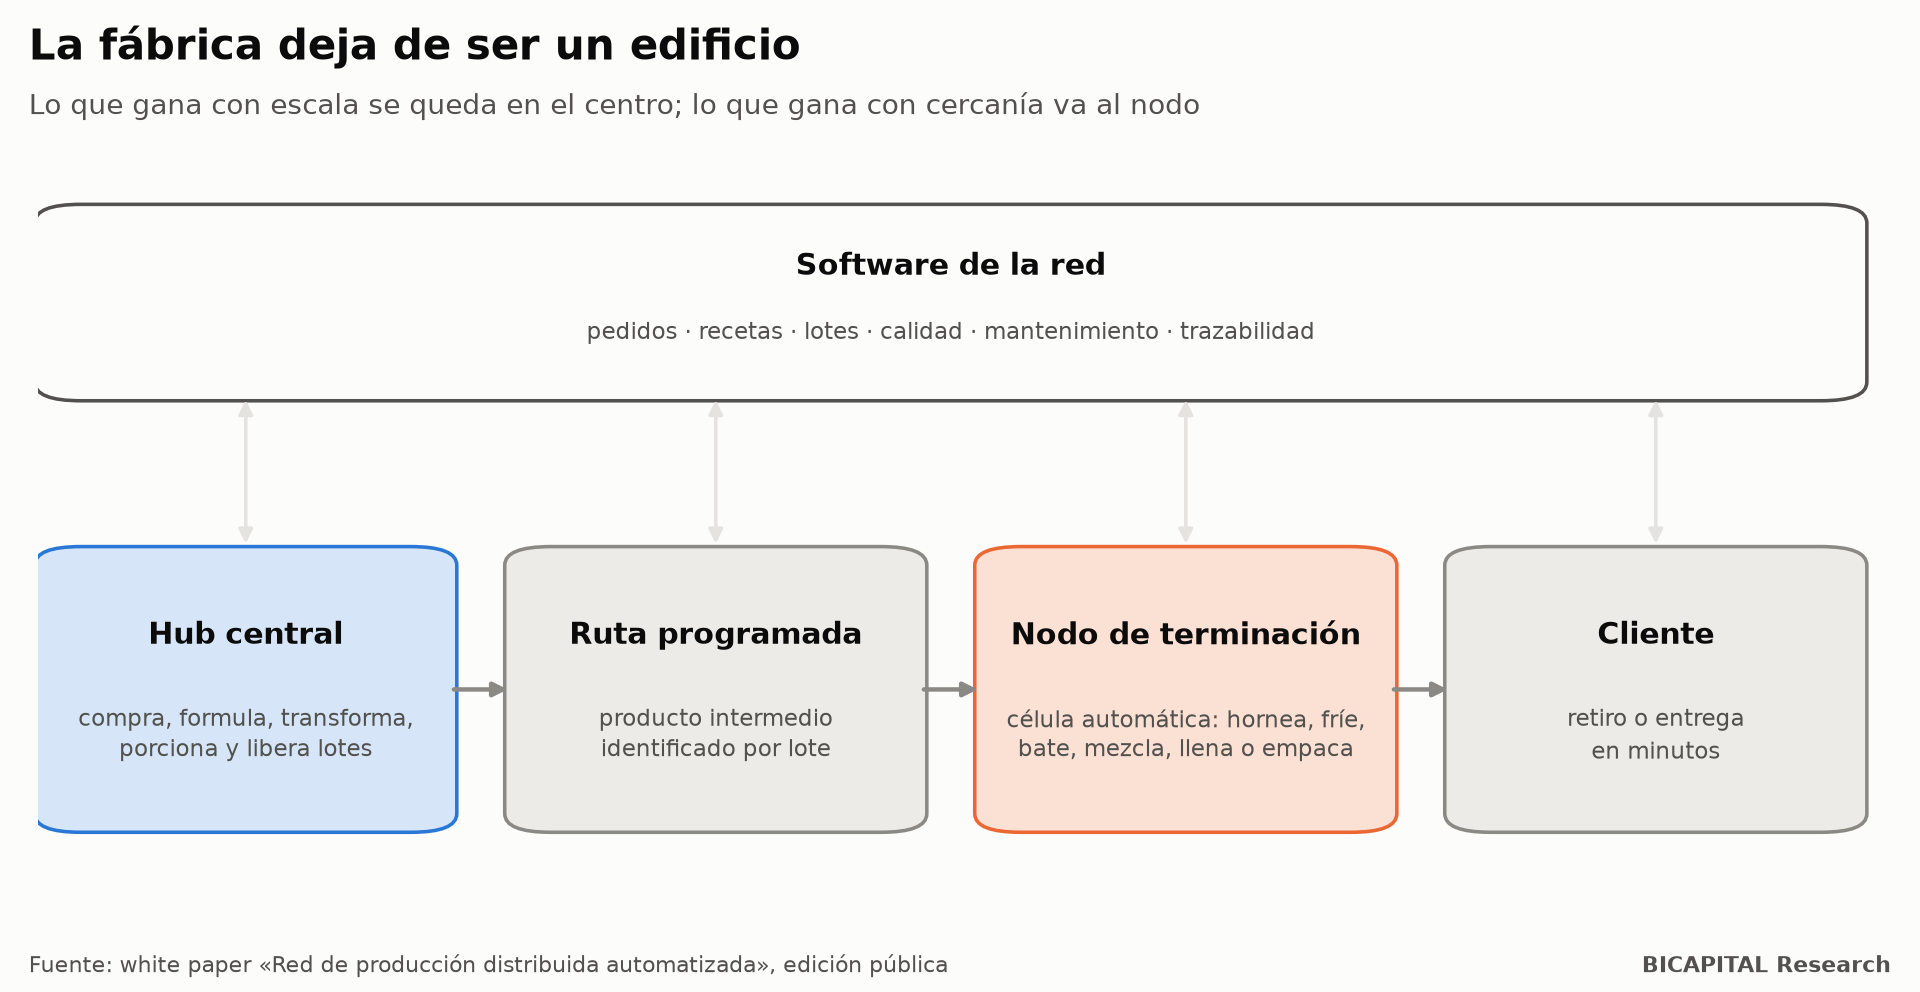
\includegraphics[width=\textwidth]{E02_arquitectura.png}
\caption{Arquitectura general de la red: hub central, ruta, nodo de terminación y software.}
\label{fig:arquitectura}
\end{figure}

La figura~\ref{fig:arquitectura} resume los componentes que se describen a continuación.

\subsubsection*{A. Hub Central de Transformación (HCT)}
El hub central compra a escala, reduce dispersión de proveedores, controla especificaciones, ejecuta los
procesos que requieren infraestructura, conocimiento o inspección avanzada y produce un intermedio
diseñado para la red. En alimentos puede recibir materias primas, lavar, clasificar, formular,
pasteurizar, marinar, cocinar parcialmente, congelar, porcionar y empacar. En productos de limpieza puede
fabricar concentrados. En cosmética puede producir bases. En manufactura puede preparar blanks, kits o
componentes.
\begin{itemize}
\item Plan maestro de producción basado en demanda agregada.
\item Laboratorio y liberación de lotes.
\item Gestión de alérgenos, trazabilidad y producto no conforme.
\item Empaque intermedio orientado a alimentación automática o semiautomática.
\item Inventario de seguridad y programación de rutas.
\item Centro de mantenimiento, repuestos y reconfiguración de células.
\end{itemize}

\subsubsection*{B. Nodo de Terminación Automatizada (NTA)}
El nodo es una unidad comercial-productiva. Su tamaño se define por proceso, no por formato de
restaurante. Puede operar sin salón y con retiro o delivery. La arquitectura debe reducir al mínimo la
manipulación abierta, el número de utensilios, la limpieza compleja y las decisiones del operador.
Idealmente el nodo trabaja con cartuchos, bolsas, bandejas o kits identificados y una célula que aplica la
receta correcta.

\subsubsection*{C. Sistema Operativo de Red Productiva (SORP)}
El SORP es el plano de control. No es un ERP genérico; es el sistema que conoce la relación entre orden,
producto, lote, receta, máquina, operador, evidencia y entrega. Debe poder bloquear un ciclo si el lote no
corresponde, cargar parámetros autorizados, registrar temperatura o peso, pedir fotografía final, emitir
etiqueta y descontar inventario. Con el tiempo incorpora pronóstico, mantenimiento predictivo, visión,
soporte asistido e inteligencia para asignar pedidos entre nodos.

\subsubsection*{D. Red logística}
La logística no desaparece; cambia de objeto. En vez de mover el producto final desde una planta nacional
a cada consumidor, mueve intermedios estandarizados desde el hub a nodos cercanos. La frecuencia y
densidad de ruta se vuelven variables centrales. El diseño debe considerar cadena de frío, retornables,
recuperación de residuos, reposición de empaques y mantenimiento preventivo. En Ecuador, la operación de
alimentos procesados debe revisar el régimen de permiso de transporte de ARCSA; el instructivo vigente
señala una vigencia anual y requisitos documentales para los vehículos sujetos a la obligación. [EXT-06]

\subsubsection*{E. Canal comercial y marca}
El sistema centraliza marketing, reputación, catálogo, promociones y datos de demanda. Los nodos pueden
recibir pedidos desde una app propia, web, WhatsApp, marketplaces o retiro. La plataforma decide qué nodo
atiende según zona, inventario, carga, SLA y calidad. La promoción no se limita a “comida barata”; debe
vender consistencia, velocidad, disponibilidad local y una experiencia visible de producción tecnológica.

\subsection{Propiedad de activos}
{\small
\begin{xltabular}{\textwidth}{@{}P{3.4cm}LL@{}}
\toprule
\textbf{Activo} & \textbf{Propietario recomendado al inicio} & \textbf{Evolución posible}\\ \midrule
Marca y recetas & Empresa central & Siempre central o licenciado de forma controlada.\\
Célula productiva & Empresa central o vehículo de leasing & Arrendamiento, lease-to-own o venta con contrato de suministro.\\
Software y datos & Empresa central & Servicio obligatorio por nodo.\\
Inventario intermedio & Central hasta entrega / consignación selectiva & Consignación según madurez del operador.\\
Local o espacio & Operador o empresa & Modelo flexible.\\
Equipos auxiliares & Estándar homologado; puede ser del operador & Lista cerrada de modelos compatibles.\\
Delivery & Terceros + flota selectiva & Orquestación híbrida según densidad.\\
\bottomrule
\end{xltabular}}

\subsection{Tipos de nodo}
El nodo domiciliario es la forma de menor CAPEX, pero no debe ser el primer formato por defecto. En
Ecuador, la compatibilidad de uso del suelo, el permiso municipal y el permiso sanitario dependen de la
actividad y del establecimiento. En Quito, la LUAE es el permiso para ejercer actividades económicas en un
establecimiento y el municipio exige verificar previamente la compatibilidad de uso de suelo.
[EXT-07][EXT-08] Por tanto, “en casa” es una hipótesis de diseño que debe convertirse en una categoría de
nodo certificable, no una excepción informal.

% =====================================================================
\section{Problema económico y operativo que resuelve}

\lead{La fábrica grande puede ser eficiente dentro de sus paredes y, al mismo tiempo, producir una cadena
total ineficiente. El SPDA busca optimizar el costo sistémico, no únicamente el costo de transformación
industrial.}

\subsection{Costos que la organización tradicional replica}
\begin{itemize}
\item \textbf{Compras fragmentadas.} Cada local negocia, recibe, inspecciona y almacena materias primas.
\item \textbf{Cocinas sobredimensionadas.} El local paga metros cuadrados, extracción, frío, gas,
utensilios y permisos para procesos que podrían estar centralizados.
\item \textbf{Talento difícil de estandarizar.} La calidad depende de entrenamiento, experiencia, rotación
y supervisión.
\item \textbf{Inventario de baja visibilidad.} Cada punto mantiene stock, merma y caducidad sin una visión
unificada.
\item \textbf{Logística de muchos proveedores.} Múltiples vehículos entregan pequeños volúmenes a cada
punto.
\item \textbf{Calidad reactiva.} Los problemas se descubren por reclamos, no por datos del proceso.
\item \textbf{CAPEX de entrada.} El franquiciado debe financiar una operación completa antes de probar
demanda.
\end{itemize}

\subsection{Ecuación de diseño}
\begin{caja}{Costo sistémico}
Costo total = transformación central + empaque intermedio + logística a nodos + costo del nodo + costo de
entrega final + merma + inventario + calidad + mantenimiento + costo de capital. El modelo gana cuando
reduce el conjunto, aunque alguna etapa individual resulte más cara.
\end{caja}

La red distribuida puede aceptar un costo de terminación local ligeramente superior si reduce
arrendamiento, inventario, tiempos, desperdicio, entrenamiento, transporte del producto terminado o
pérdidas por pronóstico. A la inversa, una célula muy sofisticada puede destruir el caso si su utilización
es baja, si requiere un técnico permanente o si los consumibles propietarios elevan el costo. Por ello, el
KPI maestro no es “número de robots”; es costo total por orden conforme y entregada.

\subsection{Fuentes de ventaja}
{\small
\begin{xltabular}{\textwidth}{@{}P{3.4cm}LL@{}}
\toprule
\textbf{Palanca} & \textbf{Mecanismo} & \textbf{Condición para que exista}\\ \midrule
\endhead
Compra y formulación central & Mayor volumen, especificación única y control de proveedor. & Demanda agregada suficiente y baja complejidad de SKU.\\
Menor área del nodo & Se eliminan bodegas, preparación pesada y parte de la cocina. & El intermedio llega listo y el equipo es compacto.\\
Automatización & Reduce variación, tiempo de capacitación y exposición a tareas calientes. & Proceso repetible y máquina mantenible.\\
Logística consolidada & Una ruta repone varios nodos. & Densidad geográfica y planificación.\\
Producción bajo pedido & Menor inventario final y mayor frescura. & Tiempo de ciclo compatible con la promesa comercial.\\
Marketing central & Una marca alimenta demanda de todos los nodos. & Economía de adquisición y control de experiencia.\\
Datos de red & Aprendizaje cruzado entre nodos. & Instrumentación y disciplina de datos.\\
Financiación de equipos & Baja la barrera del operador. & Equipo estandarizado con valor residual y mantenimiento.\\
\bottomrule
\end{xltabular}}

\subsection{Por qué el momento es diferente}
Tres tendencias hacen más viable el modelo. Primero, la oferta de automatización es más profunda y China
se ha convertido en el mayor mercado y base instalada de robótica industrial. [EXT-01][EXT-02] Segundo,
fabricantes de cobots como DOBOT y JAKA ofrecen aplicaciones de empaque, manipulación, etiquetado y
paletizado para alimentos; proveedores como Hikrobot integran visión y robots móviles; Hualian ofrece
sellado, vacío, termoformado y líneas de empaque; Techik ofrece inspección por rayos X y visión; y
Newamstar desarrolla líneas integradas y personalizadas para líquidos.
[EXT-16][EXT-18][EXT-19][EXT-22][EXT-23][EXT-24] Tercero, ya existen sistemas comerciales de cocina
digital como BOTINKIT y automatización de fritura como Miso, que demuestran que recetas, dispensación y
ciclos de cocción pueden encapsularse en equipos. [EXT-12][EXT-13][EXT-15]

La evidencia no justifica asumir autonomía total. La comida es deformable, variable y difícil de
manipular; la limpieza, el abastecimiento y las excepciones continúan requiriendo personas. La
arquitectura correcta es automatización selectiva con una interfaz humana mínima, no un humanoide
generalista como requisito de entrada.

% =====================================================================
\section{Arquitectura de la red}

\lead{El SPDA debe diseñarse como un sistema ciberfísico: producto, máquina, software, operador,
logística y regulación forman una sola arquitectura. Separarlos conduce a pilotos vistosos que no
escalan.}

\subsection{Flujo físico}
\begin{enumerate}[leftmargin=2em]
\item Demanda digital agregada por zona y franja horaria.
\item Plan de producción del hub por familia, lote y fecha.
\item Fabricación y liberación del intermedio.
\item Porcionado en formato compatible con la célula del nodo.
\item Preparación de ruta y entrega con identificación de lote.
\item Recepción y validación digital en el nodo.
\item Asignación del pedido al nodo con capacidad e inventario.
\item Carga del intermedio y ejecución automática o guiada.
\item Control de variables críticas y liberación del ciclo.
\item Empaque, etiqueta, despacho y cierre de inventario.
\item Devolución de retornables, residuos o productos no conformes.
\end{enumerate}

\subsection{Flujo de información}
Cada orden debe conservar una genealogía digital: pedido, nodo, operador, lote de intermedio, versión de
receta, identificación de máquina, parámetros ejecutados, eventos, evidencia de calidad, empaque y
entrega. Esta estructura permite retirar lotes, investigar reclamos, comparar nodos y mejorar el proceso.
La trazabilidad no se agrega al final; es parte del diseño de datos.

\subsection{Arquitectura de seguridad}
\begin{itemize}
\item \textbf{Seguridad alimentaria o de producto.} Límites críticos, liberación de lotes, alérgenos,
limpieza, agua, plagas, trazabilidad y producto no conforme.
\item \textbf{Seguridad funcional.} Interlocks, guardas, paro de emergencia, control de
temperatura/presión y separación de funciones críticas respecto de la IA.
\item \textbf{Ciberseguridad.} Identidades, certificados de dispositivo, actualizaciones firmadas,
segmentación de red, logs y modo seguro offline.
\item \textbf{Continuidad.} Operación degradada ante caída de internet, respaldo de energía para control y
frío, stock de repuestos y procedimiento de sustitución.
\item \textbf{Fraude y desvío.} Inventario por lote, conciliación de consumo, cámaras en puntos críticos
cuando sea legítimo, sellos y alertas de apertura.
\item \textbf{Protección de datos.} Minimización de datos personales, control de acceso, retención y
cumplimiento de la normativa aplicable.
\end{itemize}

\subsection{Reglas de diseño del nodo}
{\small
\begin{xltabular}{\textwidth}{@{}P{4.2cm}L@{}}
\toprule
\textbf{Regla} & \textbf{Aplicación práctica}\\ \midrule
Una sola dirección de flujo & Entrada de insumo $\rightarrow$ proceso $\rightarrow$ empaque $\rightarrow$ salida; evitar cruces entre limpio y sucio.\\
Máximo de decisiones predefinidas & El operador elige pedido autorizado; no define temperatura, tiempo o dosificación libremente.\\
Alimentación compatible & Bolsas, cartuchos, bandejas o contenedores diseñados para carga rápida y baja exposición.\\
Limpieza diseñada & Piezas desmontables sin herramienta, ciclos guiados, materiales sanitarios y registro.\\
Mantenimiento por módulos & Componentes críticos intercambiables y repuestos en Ecuador.\\
Energía conocida & Carga eléctrica, ventilación, extracción y respaldo definidos antes de homologar el sitio.\\
Trazabilidad nativa & Escaneo obligatorio de insumo, máquina y pedido.\\
Interfaz de excepción & La pantalla indica qué hacer; no deja al operador improvisar.\\
Diseño para auditoría & Superficies visibles, acceso a sensores, evidencia fotográfica y checklist remoto.\\
\bottomrule
\end{xltabular}}

% =====================================================================
\section{Método para seleccionar productos y dividir procesos}

\lead{El error más costoso sería enamorarse de una máquina y luego buscar qué vender. La secuencia
correcta es producto $\rightarrow$ demanda $\rightarrow$ proceso $\rightarrow$ punto de desacople
$\rightarrow$ célula $\rightarrow$ regulación $\rightarrow$ proveedor.}

\subsection{Filtro de elegibilidad}
{\small
\begin{xltabular}{\textwidth}{@{}P{3.4cm}L@{}}
\toprule
\textbf{Dimensión} & \textbf{Pregunta de aceptación}\\ \midrule
Demanda & Frecuente, repetible, geográficamente densa o capturable por marketing digital.\\
Producto intermedio & Puede almacenarse y transportarse de forma segura y estable.\\
Operación final & Compacta, repetible, automatizable y con tiempo compatible con delivery o retiro.\\
Valor local & La terminación cerca del cliente aporta frescura, personalización, velocidad o ahorro logístico.\\
Espacio & El nodo puede operar en menos de 50 m²; idealmente menos de 20 m² para formato domiciliario.\\
Personal & Una persona puede atender una o varias células sin habilidad especializada.\\
Limpieza & La carga de limpieza es corta, guiable y auditable.\\
Regulación & Existe una ruta razonable de permiso y control para el tipo de nodo.\\
Mantenimiento & La célula puede recuperarse de fallas sin movilizar un equipo de ingeniería completo.\\
Portafolio & La misma célula produce suficientes variantes para sostener utilización.\\
\bottomrule
\end{xltabular}}

\subsection{Matriz de prioridad}
La figura~\ref{fig:matriz} sintetiza visualmente la matriz; la tabla siguiente recoge la valoración
cualitativa de cada familia.

\begin{figure}[H]
\centering
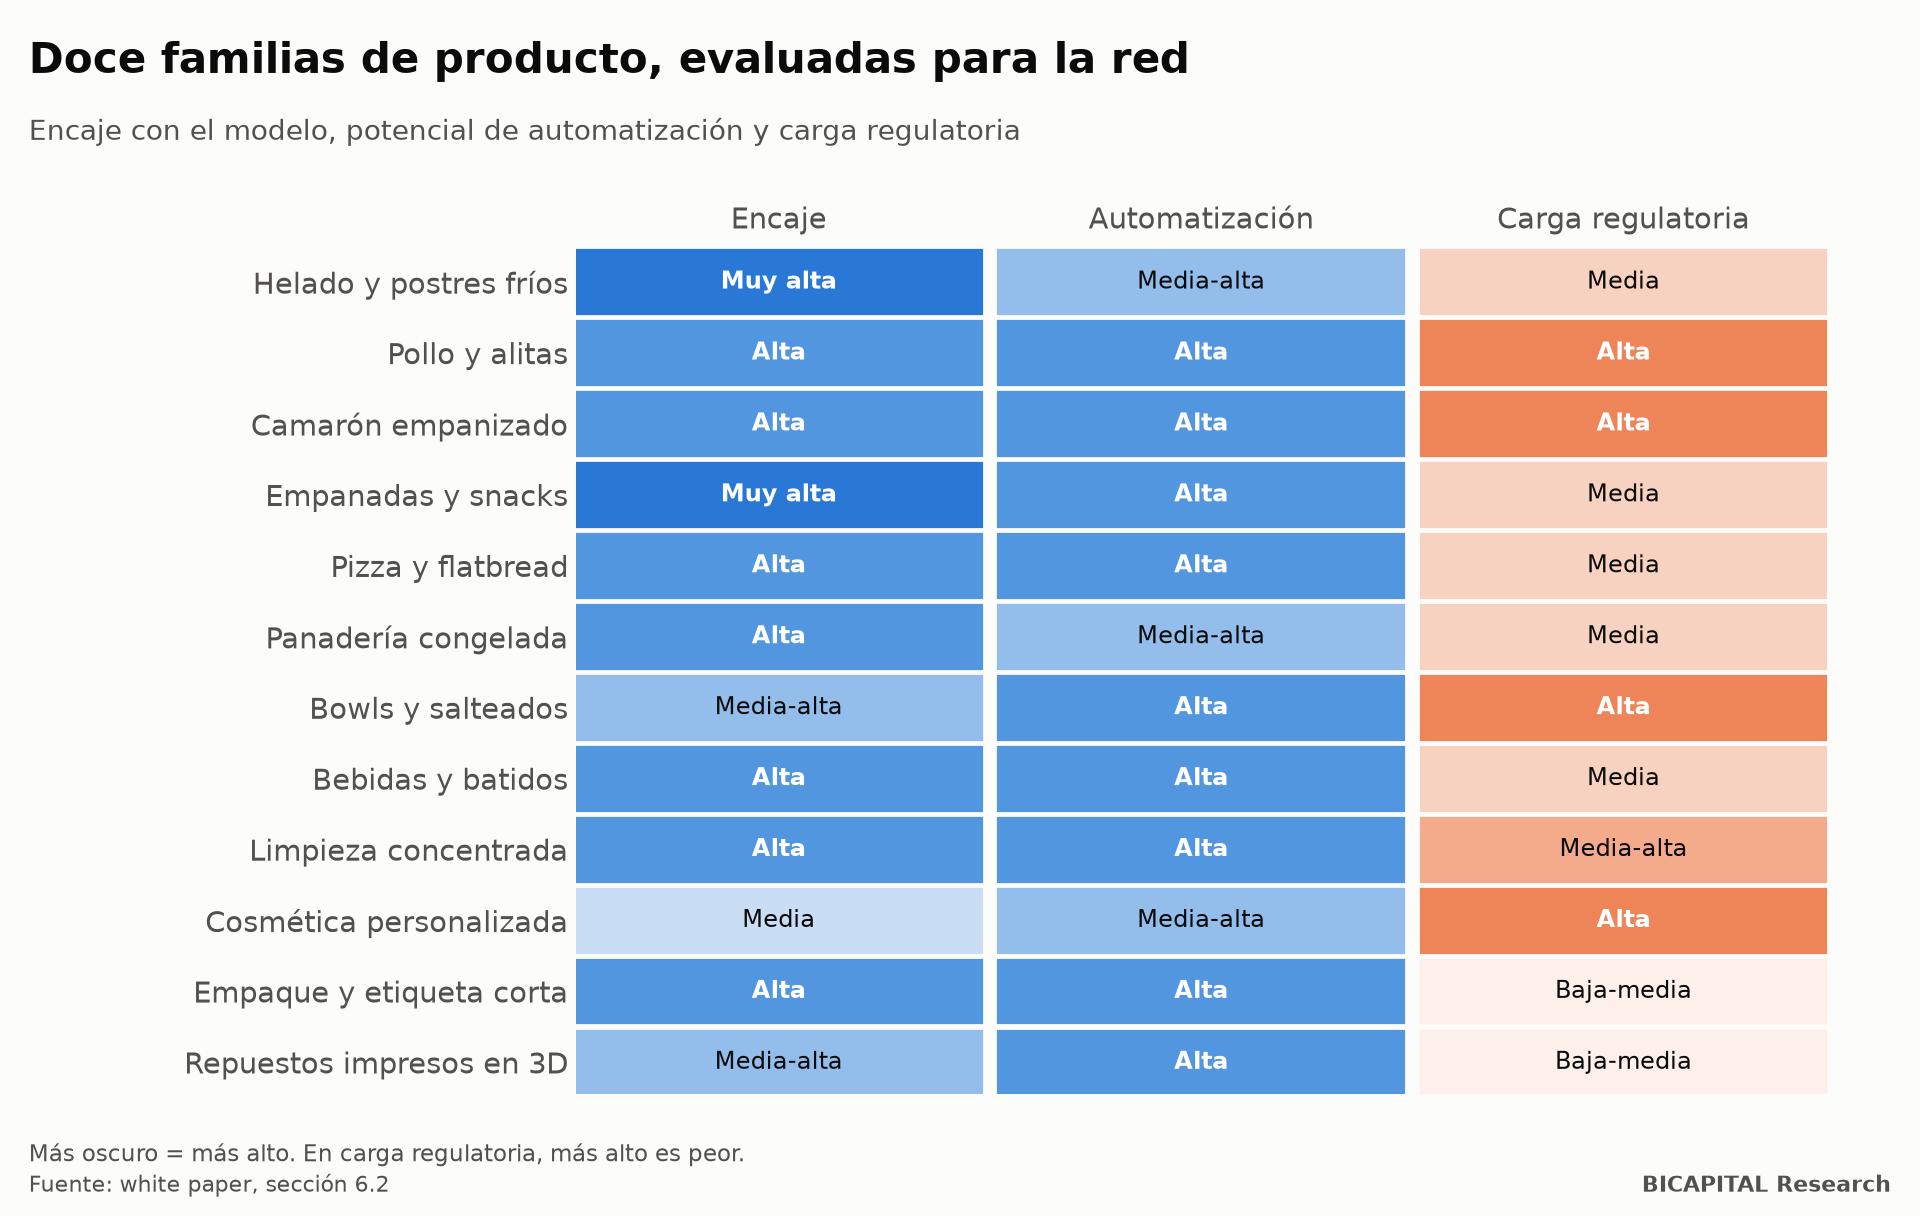
\includegraphics[width=\textwidth]{E02_matriz_familias.png}
\caption{Matriz de prioridad de las doce familias.}
\label{fig:matriz}
\end{figure}

{\footnotesize
\begin{xltabular}{\textwidth}{@{}P{2.6cm}P{1.3cm}P{2.15cm}P{1.5cm}P{2.3cm}L@{}}
\toprule
\textbf{Familia} & \textbf{Ajuste} & \textbf{Automati\-zación} & \textbf{Carga regulatoria} & \textbf{Nodo inicial} & \textbf{Razón}\\ \midrule
\endhead
Helado y postres fríos & Muy alta & Media-Alta & Media & Microlocal / corner & Producción central y cadena de frío habituales en la industria; producto atractivo y demostrable.\\
Pollo/wings terminados & Alta & Alta & Alta & Microlocal & Demanda masiva; alto valor de automatizar fritura, pero mayor riesgo sanitario.\\
Camarón empanizado & Alta & Alta & Alta & Microlocal & Ventaja ecuatoriana de materia prima; cadena de frío y alérgenos críticos.\\
Empanadas y snacks & Muy alta & Alta & Media & Domiciliario certificado / microlocal & Intermedio congelado estable; finalización simple y portafolio amplio.\\
Pizza/flatbread & Alta & Alta & Media & Microlocal / corner & Conveyor oven y kits estandarizados; demanda digital fuerte.\\
Panadería congelada & Alta & Media-Alta & Media & Domiciliario certificado / corner & Horneado local aporta aroma y frescura; ciclo más largo.\\
Wok/bowls & Media-Alta & Alta & Alta & Microlocal & La cocina digital existe, pero exige ingredientes y limpieza bien diseñados.\\
Bebidas y smoothies & Alta & Alta & Media & Corner / domiciliario & Pods congelados y dispensación reducen complejidad.\\
Limpieza concentrada & Alta & Alta & Media-Alta & Microlocal industrial & Buena economía logística; no asumir uso domiciliario.\\
Cosmética personalizada & Media & Media-Alta & Alta & Microlocal especializado & Margen y personalización; regulación y estabilidad requieren control.\\
Empaque/\allowbreak etiqueta corta & Alta & Alta & Baja-Media & Microlocal & Demanda B2B local; producción digital y bajo inventario.\\
Repuestos impresos 3D & Media-Alta & Alta & Baja-Media & Microlocal técnico & Valor por disponibilidad; requiere biblioteca validada y control dimensional.\\
\bottomrule
\end{xltabular}}

\subsection{CAPEX por bandas}
Las siguientes bandas son parámetros de ingeniería para organizar el portafolio, no cotizaciones. El
valor real depende de capacidad, acero sanitario, certificaciones, transporte, arancel, instalación,
tooling, extracción, frío, repuestos y software.

{\small
\begin{xltabular}{\textwidth}{@{}P{3.4cm}P{3.4cm}L@{}}
\toprule
\textbf{Banda} & \textbf{Orden de magnitud} & \textbf{Tipo de célula}\\ \midrule
A -- Demostrador & USD 3.000--15.000 & Equipo comercial programable + sensórica + interfaz; útil para validar receta y flujo.\\
B -- Nodo compacto & USD 15.000--50.000 & Célula integrada de una operación principal con empaque básico.\\
C -- Nodo automatizado & USD 50.000--150.000 & Múltiples módulos, alimentación, visión, seguridad y conectividad industrial.\\
D -- Hub/multicélula & Más de USD 150.000 & Línea central o nodo de alta capacidad; requiere ingeniería y RFQ formal.\\
\bottomrule
\end{xltabular}}

\begin{figure}[H]
\centering
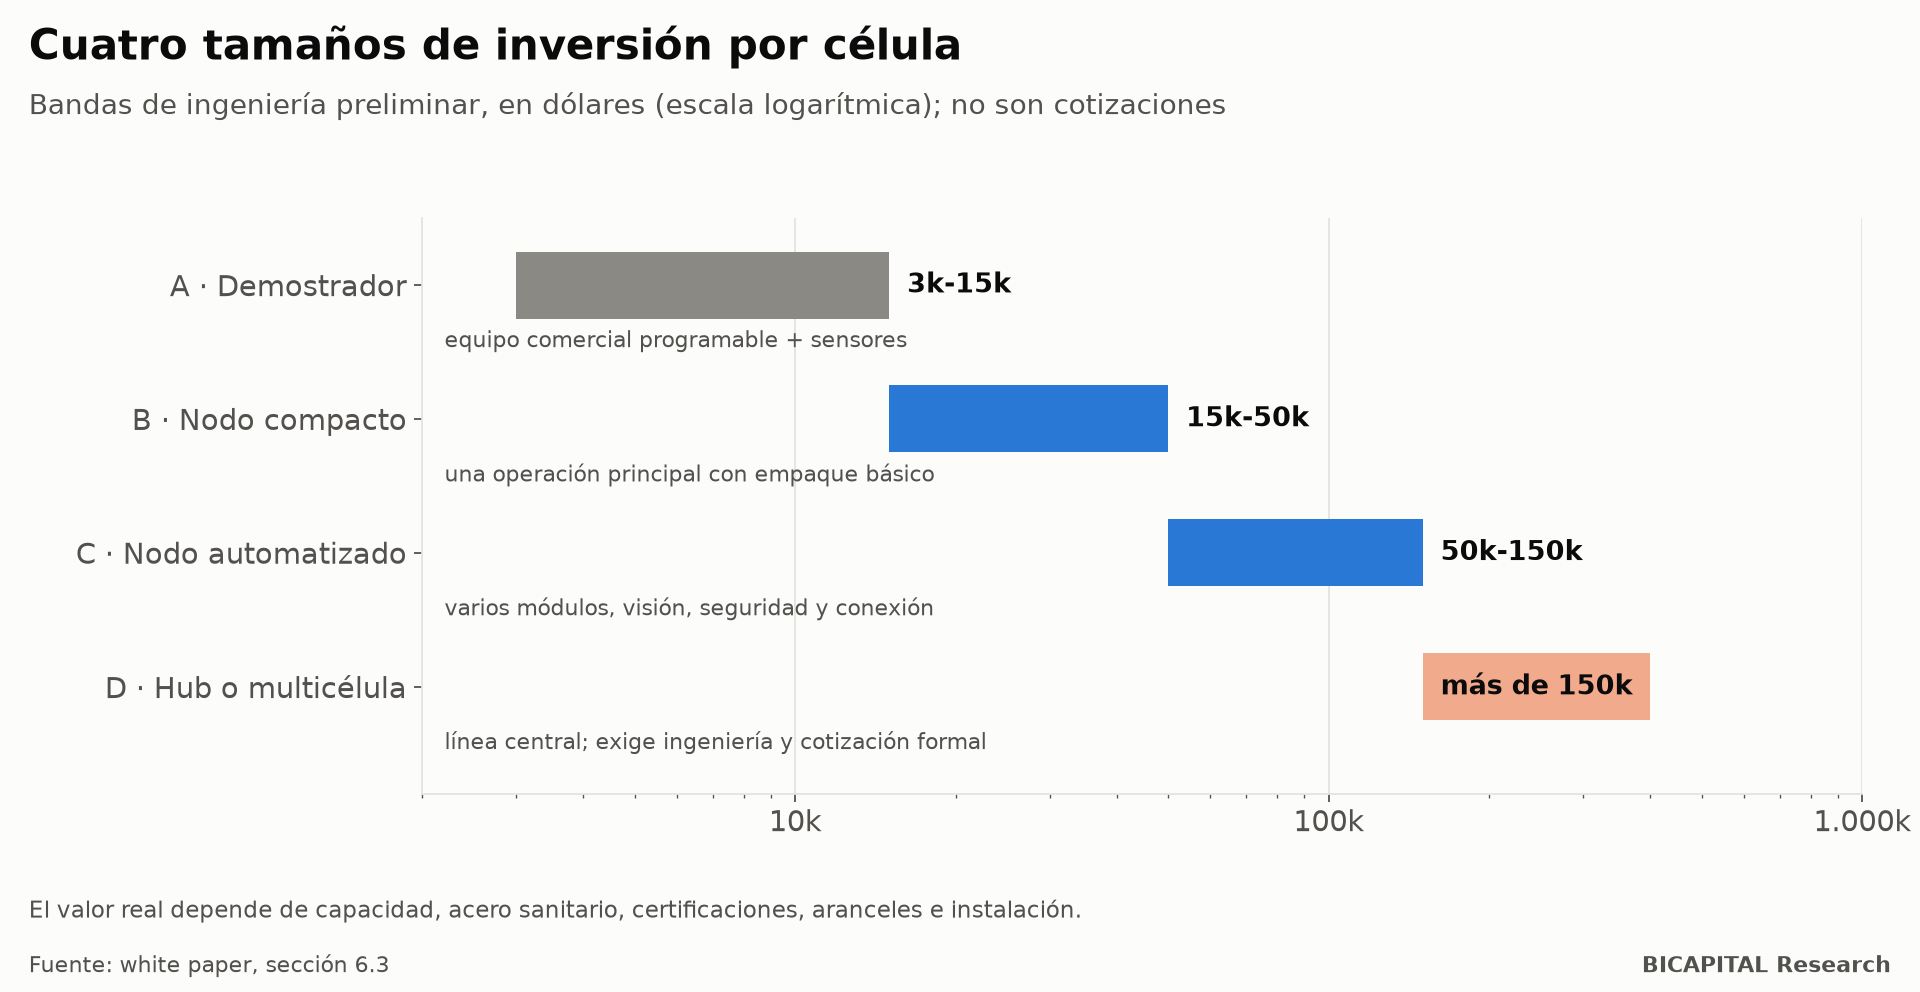
\includegraphics[width=\textwidth]{E02_capex.png}
\caption{Bandas de CAPEX por tipo de célula.}
\label{fig:capex}
\end{figure}

% =====================================================================
\section{Casos implementables en Ecuador}

\lead{Los casos siguientes no son planes financieros. Son arquitecturas implementables que muestran cómo
dividir el proceso, qué célula se requiere, qué operador sería adecuado y cuáles son los gates técnicos y
regulatorios.}

% ---------------------------------------------------------------------
\subsection{Helado y postres fríos terminados localmente}
Es un caso de entrada lógico cuando un productor ya dispone de formulación, cadena de frío y
distribución mayorista: existe capacidad productiva, experiencia en formulación y distribución, y una red
de clientes que puede servir para entrevistas, pruebas y selección de ubicaciones.

\desacople{%
\ti Compra y recepción de leche, pulpas, azúcares, estabilizantes y empaques.
\ti Formulación, mezcla, pasteurización, homogeneización y maduración según producto.
\ti Producción de base líquida refrigerada, concentrado o base congelada, definida por estudios de vida útil.
\ti Dosificación en bolsas o cartuchos identificados por lote y sabor.
\ti Liberación de calidad, cadena de frío y despacho.}{%
\ti Escaneo de base y orden.
\ti Carga en batch freezer compacto, mantecadora o equipo de soft-serve homologado.
\ti Adición automática o guiada de inclusiones autorizadas.
\ti Extrusión, porcionado o llenado de envase.
\ti Control de peso, temperatura y apariencia.
\ti Empaque, etiqueta y entrega.}

\etiqueta{Célula mínima viable}
Refrigeración de recepción; lector QR; mantecadora/batch freezer o sistema de soft-serve; dosificador de
inclusiones; balanza conectada; selladora/etiquetadora; congelador de mantenimiento; HMI y gateway edge.

\etiqueta{Formato de nodo recomendado}
Corner en cafetería, microlocal de 10--25 m² o nodo de delivery. El domicilio puede evaluarse después de
validar compatibilidad de uso, separación sanitaria, energía, agua y permisos.

\etiqueta{Gates antes de escalar}
\begin{itemize}
\item Definir científicamente el intermedio: composición, temperatura, vida útil y estabilidad.
\item Determinar si el producto se considera fabricado en el hub, terminado en el nodo o elaborado en
ambos para efectos de permisos y trazabilidad.
\item Validar tiempo por pedido y capacidad de congelación en horas pico.
\item Diseñar limpieza de la máquina sin desmontajes complejos.
\item Probar una familia corta de sabores para maximizar utilización.
\end{itemize}

\rutas{Equipo comercial programable, operación guiada y pesaje digital.}
{Carga por cartucho, dosificación automática e integración con pedidos.}
{Visión de porción, autolimpieza parcial y asignación dinámica de producción.}

\etiqueta{Modelo comercial}
La empresa central vende base y empaques, arrienda la célula, cobra software/soporte y participa en la
venta final. El operador aporta espacio, energía, atención y despacho.

\criterio

% ---------------------------------------------------------------------
\subsection{Pollo crujiente, wings y tenders de terminación automática}
El valor no está en que cada punto compre pollo crudo, marine, empanice y gestione una cocina completa. El
hub puede recibir volumen, especificar cortes, marinar, empanizar, cocinar parcialmente o congelar y
entregar un intermedio que el nodo solo termina. La automatización de fritura ya se despliega
comercialmente; Miso presenta una plataforma de estación de fritura utilizada por cadenas, mientras que
proveedores chinos comercializan cocción programada y pueden desarrollar equipos OEM. [EXT-15]

\desacople{%
\ti Recepción de pollo bajo especificación.
\ti Desposte, porcionado y control de rendimiento.
\ti Marinado al vacío o por tambor.
\ti Empanizado y, según validación, prefritura o cocción completa seguida de congelación rápida.
\ti Empaque por raciones y lote.
\ti Liberación microbiológica y logística congelada.}{%
\ti Recepción congelada y almacenamiento.
\ti Carga de una ración cerrada o cesta identificada.
\ti Ciclo automático de fritura/horneado con control de tiempo y temperatura.
\ti Escurrido o manejo automático de aceite.
\ti Dosificación de salsa o sazonado.
\ti Empaque y despacho.}

\etiqueta{Célula mínima viable}
Congelador; estación automática de fritura o horno de alta velocidad; filtrado de aceite; extracción;
dosificador de salsa; mesa de empaque; balanza; sensor de temperatura; HMI y bloqueo de recetas.

\etiqueta{Formato de nodo recomendado}
Microlocal de 15--35 m². No se recomienda como primer nodo domiciliario por carga térmica, extracción,
aceite, residuos, manipulación de proteína y permisos.

\etiqueta{Gates antes de escalar}
\begin{itemize}
\item Elegir un intermedio que minimice riesgo en el nodo: preferir producto completamente cocido o
validado para retermalización cuando sea compatible con calidad.
\item Validar capacidad de extracción, potencia y protección contra incendio.
\item Establecer control de aceite, vida útil, filtrado y disposición.
\item Diseñar empaque para delivery sin pérdida excesiva de textura.
\item Separar alérgenos y contaminación cruzada.
\end{itemize}

\rutas{Freidora programable con recetas bloqueadas y registro de ciclos.}
{Carga/descarga semiautomática, filtrado automático y dosificación.}
{Célula cerrada con visión, empaque integrado y operación multicanal.}

\etiqueta{Modelo comercial}
Formato de marca propia o marca virtual. La empresa controla producto intermedio, receta, aceite
homologado, empaques, marketing y canal; el operador ejecuta y despacha.

\criterio

% ---------------------------------------------------------------------
\subsection{Camarón empanizado y snacks de mar}
Ecuador posee una cadena exportadora de camarón y conocimiento del producto. Una red local podría capturar
valor en presentaciones de consumo rápido, mientras el hub ejecuta clasificación, limpieza, sazonado,
empanizado y congelación. La terminación local preserva textura y reduce la necesidad de cocinas
completas.

\desacople{%
\ti Abastecimiento por calibre y especificación.
\ti Desvenado/limpieza cuando corresponda.
\ti Sazonado, marinado o preformado.
\ti Empanizado, prefritura opcional y congelación rápida.
\ti Porciones monopedido o multipedido.
\ti Control de alérgenos, temperatura y vida útil.}{%
\ti Escaneo de lote y selección de pedido.
\ti Fritura, air-fry u horneado automático.
\ti Dosificación de salsas y acompañamientos.
\ti Control de peso y empaque ventilado.
\ti Despacho por delivery o retiro.}

\etiqueta{Célula mínima viable}
Congelador; freidora/horno programable; extracción; dosificador de salsa; selladora o estación de
empaque; balanza conectada; sensores y HMI.

\etiqueta{Formato de nodo recomendado}
Microlocal o dark node de 12--30 m² cerca de zonas residenciales y oficinas. Puede compartir plataforma
con pollo si se diseña segregación estricta de alérgenos y protocolos.

\etiqueta{Gates antes de escalar}
\begin{itemize}
\item No mezclar líneas sin validar control de alérgeno crustáceo.
\item Asegurar textura después del tiempo real de delivery.
\item Definir política de aceite y evitar transferencia de sabor.
\item Validar proveedor, glaseado, rendimiento y mermas.
\item Incluir trazabilidad robusta por lote.
\end{itemize}

\rutas{Producto congelado porcionado + equipo programable.}
{Cestas inteligentes, dosificación y empaque guiado.}
{Célula cerrada compartida con múltiples snacks, con secuencia y limpieza automatizadas.}

\etiqueta{Modelo comercial}
Marca premium-accesible de snacks de mar; nodo con bajo menú, alta velocidad y fuerte marketing digital.
El hub captura margen de transformación y suministro.

\criterio

% ---------------------------------------------------------------------
\subsection{Empanadas, deditos, croquetas y snacks congelados}
Es una de las familias más compatibles con el modelo. El hub puede formar y congelar productos de muchas
recetas; el nodo solo hornea o fríe. La variedad comercial se obtiene sin multiplicar equipos ni
habilidades. Es candidato a nodo domiciliario certificado después de validar regulación y diseño
sanitario.

\desacople{%
\ti Producción de masas y rellenos.
\ti Formado, sellado y control de peso.
\ti Prefritura cuando aplique.
\ti Congelación y empaque por SKU/lote.
\ti Liberación y despacho consolidado.}{%
\ti Recepción congelada.
\ti Carga por bandeja o cesta.
\ti Ciclo automático según SKU.
\ti Sazonado o acabado simple.
\ti Conteo, empaque y entrega.}

\etiqueta{Célula mínima viable}
Congelador vertical; horno de convección/conveyor o freidora programable; bandejas/cestas codificadas;
extractor según tecnología; temporización, temperatura y HMI; selladora/etiquetadora.

\etiqueta{Formato de nodo recomendado}
Domiciliario certificado de 6--15 m², corner de tienda o microlocal. Es apropiado para operadores que
trabajan desde casa si el establecimiento puede cumplir requisitos físicos, municipales y sanitarios.

\etiqueta{Gates antes de escalar}
\begin{itemize}
\item Compatibilidad de uso de suelo y permiso del establecimiento.
\item Separación física del área doméstica.
\item Control de frío y respaldo.
\item Diseño de limpieza y manejo de aceite.
\item Canal digital capaz de consolidar demanda en radio corto.
\end{itemize}

\rutas{Horno/freidora programable + app de pedidos.}
{Bandejas identificadas, dosificación y empaque asistido.}
{Carga automática, visión de color y conteo, despacho en lockers.}

\etiqueta{Modelo comercial}
Microfranquicia de baja inversión con equipo en arrendamiento, kit de apertura y suministro obligatorio.
Puede operar una marca o un portafolio de marcas virtuales sobre la misma célula.

\criterio

% ---------------------------------------------------------------------
\subsection{Pizza, flatbread y productos horneados de alta rotación}
La pizza combina demanda digital, posibilidad de preprocesar masa y salsa, equipos compactos y cocción
estandarizable. El nodo puede ser visible al cliente y funcionar con poco personal. La automatización
completa del topping no es necesaria en la primera versión; la clave es estandarizar kits y horneado.

\desacople{%
\ti Masa o base prehorneada según diseño.
\ti Salsa, quesos y toppings porcionados.
\ti Kits por tamaño/receta.
\ti Pruebas de fermentación, estabilidad y vida útil.
\ti Empaque de componentes y despacho refrigerado/congelado.}{%
\ti Escaneo de kit.
\ti Armado guiado o dosificación semiautomática.
\ti Horneado en conveyor o horno rápido con receta bloqueada.
\ti Corte, empaque y despacho.}

\etiqueta{Célula mínima viable}
Refrigeración; mesa fría compacta; dosificadores de salsa/queso opcionales; horno conveyor o de alta
velocidad; cortador/guía; caja y etiqueta; HMI.

\etiqueta{Formato de nodo recomendado}
Corner, microlocal o dark node de 12--30 m². Puede operar en zonas de alta demanda nocturna y compartir
logística con otras familias congeladas.

\etiqueta{Gates antes de escalar}
\begin{itemize}
\item Comparar masa fresca, congelada y base prehorneada.
\item Asegurar uniformidad de armado sin chef.
\item Validar tiempo total en hora pico.
\item Diseñar ventilación y carga eléctrica/gas.
\item Controlar inventario de toppings para evitar complejidad.
\end{itemize}

\rutas{Kit porcionado + horno programable.}
{Dispensación semiautomática y visión de cobertura.}
{Estación automática de armado y horneado continuo.}

\etiqueta{Modelo comercial}
Marca digital con menú corto y alto uso de promociones; célula financiada por la central y
abastecimiento periódico.

\criterio

% ---------------------------------------------------------------------
\subsection{Panadería y masas congeladas: hornear cerca del consumidor}
La industria ya utiliza masa congelada y bake-off. La oportunidad es llevar el modelo a nodos pequeños con
programación, control y marketing central. El aroma y la frescura se generan localmente; el proceso
complejo de formulación y formado permanece en el hub.

\desacople{%
\ti Mezcla y amasado.
\ti División, formado y fermentación controlada.
\ti Congelación de masa cruda, prefermentada o prehorneada.
\ti Empaque por bandeja y SKU.
\ti Pruebas de vida útil y desempeño.}{%
\ti Descongelación/fermentación programada si aplica.
\ti Horneado automático por receta.
\ti Acabado simple: glaseado, relleno o empaque.
\ti Exhibición, retiro o delivery.}

\etiqueta{Célula mínima viable}
Congelador; fermentadora compacta; horno programable con vapor; carros/bandejas estandarizados; sensor de
humedad/temperatura; mesa de acabado; empaque.

\etiqueta{Formato de nodo recomendado}
Corner en tienda, cafetería, estación o domicilio certificado con área separada. Es más adecuado para
producción programada por franjas que para demanda instantánea.

\etiqueta{Gates antes de escalar}
\begin{itemize}
\item Sincronizar tiempo de fermentación con demanda.
\item Evitar exceso de SKU.
\item Asegurar ventilación y potencia.
\item Diseñar gestión de sobrantes.
\item Validar textura después de empaque y delivery.
\end{itemize}

\rutas{Programación de lotes y horno conectado.}
{Fermentación automatizada y forecast por nodo.}
{Carga de bandejas robotizada en hubs urbanos de mayor volumen.}

\etiqueta{Modelo comercial}
Suministro de masa congelada + arrendamiento de horno + plataforma de demanda. Puede coexistir con
tiendas existentes sin crear un local nuevo.

\criterio

% ---------------------------------------------------------------------
\subsection{Bowls, arroces y salteados mediante cocina digital}
Los equipos de cocina digital demuestran que una receta puede convertirse en secuencias de temperatura,
agitación y dosificación. BOTINKIT promociona equipos con control automático, dispensación precisa y
recetas gestionadas en la nube. [EXT-12][EXT-13][EXT-14] El modelo encaja si el hub prepara componentes y
el nodo realiza la cocción final bajo pedido.

\desacople{%
\ti Corte, lavado y porcionado de proteínas y vegetales.
\ti Producción de salsas y bases.
\ti Precocción de arroz o granos cuando sea tecnológicamente adecuada.
\ti Kits por receta o componentes en cartuchos.
\ti Control de vida útil y cadena de frío.}{%
\ti Carga de ingredientes o cartuchos.
\ti Cocción automática en wok/tambor/pan con dosificación.
\ti Descarga al envase.
\ti Topping y empaque.
\ti Limpieza automática o semiautomática entre ciclos.}

\etiqueta{Célula mínima viable}
Robot/cocedor de wok o tambor; dispensadores líquidos/sólidos; refrigeración de cartuchos; extractor;
estación de empaque; HMI; sistema de lavado.

\etiqueta{Formato de nodo recomendado}
Microlocal de 15--35 m². La operación domiciliaria requiere evaluación estricta por extracción, agua,
limpieza, residuos y complejidad de ingredientes.

\etiqueta{Gates antes de escalar}
\begin{itemize}
\item Reducir número de componentes abiertos.
\item Validar limpieza entre alérgenos y sabores.
\item Medir capacidad real en hora pico con tiempos de lavado.
\item Diseñar recetas que toleren variación de materia prima.
\item Asegurar disponibilidad de repuestos y soporte local.
\end{itemize}

\rutas{Cocedor digital con carga manual estandarizada.}
{Cartuchos y dosificación automática.}
{Alimentación robotizada, visión y multicocción coordinada.}

\etiqueta{Modelo comercial}
Marca digital de bowls accesibles con receta centralizada. La célula puede atender varias marcas
virtuales que compartan bases e ingredientes.

\criterio

% ---------------------------------------------------------------------
\subsection{Smoothies, jugos, bebidas y postres de fruta}
Ecuador posee diversidad de frutas y una base agroindustrial. El hub puede transformar pulpa, controlar
formulación y congelar pods; el nodo mezcla, dosifica y entrega. El proceso final es compacto y visual,
adecuado para corners, gimnasios, universidades y nodos domiciliarios certificados.

\desacople{%
\ti Compra y selección de fruta/pulpa.
\ti Lavado, pulpeado, formulación y tratamiento requerido.
\ti Producción de pods congelados o bolsas monodosis.
\ti Control de °Brix, acidez, microbiología y vida útil.
\ti Despacho congelado.}{%
\ti Escaneo de pod.
\ti Carga automática o manual en blender cerrado.
\ti Adición dosificada de agua/leche/base.
\ti Mezcla, llenado y sellado.
\ti Limpieza automática del vaso de proceso.}

\etiqueta{Célula mínima viable}
Congelador; blender industrial cerrado; dispensadores; estación de vasos; selladora de film;
balanza/medidor; HMI y sistema de lavado.

\etiqueta{Formato de nodo recomendado}
Corner de 4--10 m², kiosco, gimnasio, universidad o domicilio certificado. Puede operar con una persona y
alta automatización.

\etiqueta{Gates antes de escalar}
\begin{itemize}
\item Controlar cadena de frío y descongelamiento.
\item Diseñar ciclo de lavado rápido y seguro.
\item Evitar proliferación de recetas que complique inventario.
\item Validar empaque para delivery.
\item Clasificar regulatoriamente el producto final y el intermedio.
\end{itemize}

\rutas{Pods + blender programable.}
{Dosificación y sellado integrados.}
{Kiosco autónomo con reposición y monitoreo remoto.}

\etiqueta{Modelo comercial}
Venta por suscripción, oficinas y retail; arrendamiento de célula y suministro de pods. Puede aprovechar
pulpas y know-how de un productor de helados en una familia adyacente.

\criterio

% ---------------------------------------------------------------------
\subsection{Productos de limpieza a partir de concentrados}
La lógica no alimentaria es potente: transportar agua en productos terminados puede ser ineficiente. El
hub produce concentrados y controla formulación; nodos industriales pequeños diluyen, dosifican, llenan y
etiquetan cerca del mercado. ARCSA dispone de simuladores y trámites para productos de higiene doméstica,
por lo que la clasificación y autorización deben estudiarse desde el inicio. [EXT-03]

\desacople{%
\ti Formulación y fabricación de concentrados.
\ti Control fisicoquímico y estabilidad.
\ti Envasado de concentrados en contenedores seguros.
\ti Gestión de etiquetas, fichas y lotes.}{%
\ti Conexión de concentrado y agua tratada.
\ti Dosificación automática y mezcla cerrada.
\ti Llenado, tapado y etiquetado.
\ti Control de peso y lote.
\ti Empaque para retail o entrega B2B.}

\etiqueta{Célula mínima viable}
Tratamiento/medición de agua; skid cerrado de dosificación; mezclador; llenadora; tapadora;
etiquetadora; bandeja de contención; ventilación y HMI.

\etiqueta{Formato de nodo recomendado}
Microlocal industrial de 20--60 m² o hub urbano. No asumir operación domiciliaria por almacenamiento
químico, derrames, ventilación y regulación.

\etiqueta{Gates antes de escalar}
\begin{itemize}
\item Clasificación sanitaria y autorizaciones.
\item Compatibilidad química de materiales.
\item Control de agua y concentración.
\item Gestión de derrames, EPP y residuos.
\item Etiquetado y trazabilidad.
\end{itemize}

\rutas{Dosificación semiautomática y llenado.}
{Skid cerrado con receta digital.}
{Nodo multiformulación con inspección y reposición automática.}

\etiqueta{Modelo comercial}
Venta B2B a comercios, condominios y pequeñas empresas; modelo de refill con envases retornables y
software de reposición.

\criterio

% ---------------------------------------------------------------------
\subsection{Cosmética y cuidado personal personalizados}
La centralización de bases y la personalización local pueden reducir inventario de variantes y crear
experiencia. Sin embargo, la carga regulatoria, la estabilidad, la compatibilidad de envases y la
contaminación son altas. Es una segunda o tercera vertical, no un piloto domiciliario.

\desacople{%
\ti Fabricación de bases validadas.
\ti Ensayos de estabilidad y microbiología.
\ti Producción de concentrados de fragancia/color autorizados.
\ti Documentación técnica y lote.
\ti Empaque en cartuchos cerrados.}{%
\ti Selección de variante autorizada.
\ti Dosificación cerrada de base y concentrados.
\ti Mezcla controlada.
\ti Llenado, tapado y etiquetado.
\ti Registro de fórmula exacta y lote.}

\etiqueta{Célula mínima viable}
Dosificadores de precisión; mezclador cerrado; llenadora; tapadora; impresora/etiquetadora; balanza;
limpieza validada; HMI y trazabilidad.

\etiqueta{Formato de nodo recomendado}
Microlocal especializado o corner premium dentro de retail. No recomendado para domicilio en fase
inicial.

\etiqueta{Gates antes de escalar}
\begin{itemize}
\item Revisión de normativa de cosméticos y responsabilidad del titular.
\item Estabilidad de cada combinación.
\item Control de contaminación y limpieza.
\item Tolerancias de dosificación.
\item Gestión de claims y etiquetado.
\end{itemize}

\rutas{Personalización limitada con fórmulas preautorizadas.}
{Dosificación automática y perfil digital del cliente.}
{Recomendación asistida por IA dentro de catálogo regulado.}

\etiqueta{Modelo comercial}
Experiencia de personalización + suscripción/refill. El valor proviene de variedad virtual con
inventario físico reducido.

\criterio

% ---------------------------------------------------------------------
\subsection{Empaques, etiquetas y material promocional de tirada corta}
La producción digital de tiradas cortas es naturalmente distribuible. Un hub puede controlar diseño,
sustratos y compras; nodos locales imprimen, cortan y terminan bajo pedido. Es una vertical B2B con menor
carga sanitaria y conexión directa con la red de clientes de fabricantes de alimentos.

\desacople{%
\ti Compras de sustratos, tintas y consumibles.
\ti Biblioteca de diseños, perfiles y estándares.
\ti Preimpresión o fabricación de componentes complejos.
\ti Control de color y homologación.}{%
\ti Recepción de orden digital.
\ti Impresión/corte según archivo autorizado.
\ti Laminado o acabado simple.
\ti Inspección visual y empaque.
\ti Entrega local.}

\etiqueta{Célula mínima viable}
Impresora digital; plotter/cortadora; laminadora; mesa de acabado; cámara de inspección; software de
preflight; etiquetado y empaque.

\etiqueta{Formato de nodo recomendado}
Microlocal técnico de 15--40 m². Puede servir a restaurantes, tiendas y microempresas cercanas.

\etiqueta{Gates antes de escalar}
\begin{itemize}
\item Control de color y calibración.
\item Derechos de propiedad intelectual.
\item Inventario de sustratos.
\item Mantenimiento de cabezales y consumibles.
\item Evitar competir solo por precio.
\end{itemize}

\rutas{Producción digital bajo orden.}
{Nesting automático, visión e integración con e-commerce.}
{Red de capacidad distribuida con asignación dinámica.}

\etiqueta{Modelo comercial}
Manufacturing-as-a-Service local; tarifa por orden y suscripción B2B. La plataforma central gestiona
diseño, ventas y calidad.

\criterio

% ---------------------------------------------------------------------
\subsection{Repuestos y objetos personalizados mediante fabricación digital}
La impresión 3D y el mecanizado compacto permiten producir localmente piezas de baja serie. El valor no
está en imprimir cualquier archivo, sino en una biblioteca validada, control de material y disponibilidad
rápida. Es una extensión de la plataforma hacia manufactura ligera.

\desacople{%
\ti Ingeniería inversa y diseño.
\ti Validación de archivos, materiales y tolerancias.
\ti Biblioteca de piezas autorizadas.
\ti Compras de material y perfiles de proceso.
\ti Metrología de referencia.}{%
\ti Carga de material certificado.
\ti Fabricación según archivo firmado.
\ti Posprocesado simple.
\ti Inspección dimensional guiada.
\ti Empaque y entrega.}

\etiqueta{Célula mínima viable}
Impresora 3D industrial o CNC compacto; secado/almacenamiento de material; cámara; metrología básica;
extracción; software de colas y trazabilidad.

\etiqueta{Formato de nodo recomendado}
Microlocal técnico de 15--50 m², cerca de zonas industriales o comerciales. No es una microfranquicia de
consumo masivo; requiere operador técnico.

\etiqueta{Gates antes de escalar}
\begin{itemize}
\item Responsabilidad por falla de pieza.
\item Excluir componentes críticos sin validación.
\item Control de material, humedad y parámetros.
\item Propiedad intelectual.
\item Metrología y criterio de aceptación.
\end{itemize}

\rutas{Catálogo cerrado de piezas no críticas.}
{Visión y metrología conectada.}
{Asignación automática a red de máquinas y certificación digital de lote.}

\etiqueta{Modelo comercial}
Servicio de disponibilidad local con catálogo; cobro por pieza y SLA. La plataforma captura valor por
diseño, validación y coordinación.

\criterio

% =====================================================================
\section{Cómo empezar: un piloto sobre una operación existente}

\lead{La plataforma general debe nacer de una vertical real. Empezar sobre la operación de un productor
existente reduce el riesgo inicial porque ya existen conocimiento de producto, marca, planta, logística,
clientes y un programa BPM. El objetivo no es abandonar el negocio de ese productor, sino utilizarlo como
laboratorio operativo del sistema distribuido.}

\subsection{Activos existentes que pueden convertirse en ventaja}
Partir de un productor en marcha evita construir desde cero la planta, el conocimiento de producto, el
programa sanitario, la cartera de clientes y la logística. Cada uno de esos activos tiene un uso directo
en el piloto:

{\small
\begin{xltabular}{\textwidth}{@{}P{3.6cm}LL@{}}
\toprule
\textbf{Activo actual} & \textbf{Valor para el SPDA} & \textbf{Uso propuesto}\\ \midrule
Planta existente & Punto central de formulación, producción y despacho. & HCT piloto para bases, kits y control de calidad.\\
Experiencia productiva & Conocimiento tácito de mezcla, dosificación, producción, envasado y distribución. & Convertir conocimiento en recetas, parámetros, POE y datos.\\
Programa BPM & Estructura para higiene, limpieza, plagas, mantenimiento, bodega, alérgenos, producto no conforme y trazabilidad. & Diseñar el estándar del hub y transferir una versión específica a los nodos.\\
Base comercial de clientes mayoristas & Relación directa con comercios que ya venden el producto. & Entrevistas, pilotos, corners, ubicaciones y demanda inicial.\\
Posicionamiento como proveedor que ayuda al cliente a vender & La marca ya se presenta como aliada comercial del cliente, no solo como fabricante. & Evolucionar de vender producto a vender capacidad productiva y negocio listo.\\
Experiencia logística & Pedidos, despacho, entrega y coordinación ya forman parte de la operación. & Probar rutas de reposición de intermedios y retorno de empaques.\\
\bottomrule
\end{xltabular}}

\subsection{Dos pistas de implementación}
\begin{caja}{Pista A -- Negocio inmediato}
Nodo frío de helado/postre frío: aprovechar una planta y una cartera existentes para validar suministro
central, célula compacta, software de pedido, trazabilidad y operación con un socio.
\end{caja}
\begin{caja}{Pista B -- Demostrador tecnológico}
Nodo de snack caliente: utilizar empanadas, croquetas, deditos o un producto empanizado para demostrar
finalización automática visible, empaque rápido y delivery. Esta pista comunica mejor la promesa de
“microfábrica” y puede compartir logística congelada.
\end{caja}

\subsection{Diseño del piloto}
\begin{enumerate}[leftmargin=2em]
\item Formar un equipo núcleo: líder de negocio, ingeniería de alimentos, automatización/mecatrónica,
software y operaciones. El responsable técnico-sanitario y el programa BPM del productor pueden aportar
el marco técnico-sanitario ya iniciado.
\item Seleccionar una única familia de producto y máximo cinco SKU. La selección debe priorizar alta
rotación, proceso final visible, baja manipulación y compatibilidad con la infraestructura de frío.
\item Definir el producto intermedio con especificación: composición, tolerancias, vida útil,
temperatura, empaque, código de lote, instrucciones y criterios de rechazo.
\item Construir un demostrador con equipo comercial programable antes de mandar a fabricar una célula
OEM. El objetivo es estabilizar receta y flujo, no impresionar.
\item Instrumentar desde el primer día: escaneo de lote, receta, tiempo, temperatura, peso, operador,
foto final y entrega.
\item Operar el primer nodo bajo control directo del productor que lo impulsa durante al menos un ciclo
representativo de demanda, incluyendo fines de semana, fallas y limpieza.
\item Diseñar la célula OEM solo después de identificar movimientos, errores, tiempos muertos y puntos de
contaminación reales.
\item Abrir 3--5 nodos propios o gestionados antes de ofrecer franquicia domiciliaria. Este paso crea
manuales y evidencia de soporte.
\item Validar con ARCSA, municipio y asesoría legal la clasificación exacta del hub, el intermedio, el
nodo y el transporte antes de comercializar el formato.
\item Convertir el piloto en un paquete replicable: layout, lista de equipos, instalación, software,
capacitación, mantenimiento, auditoría y contrato.
\end{enumerate}

\subsection{Diseño de experiencia del nodo}
La automatización debe ser visible pero funcional. El cliente puede observar una célula cerrada, una
pantalla con el pedido, un temporizador, el lote y la preparación. El mensaje no debe ser “robot por
robot”; debe ser “tu pedido se produce aquí, al momento, con receta y control de fábrica”. Esto convierte
la tecnología en confianza y marketing, no solamente en ahorro interno.

\subsection{Arquitectura de marcas}
{\small
\begin{xltabular}{\textwidth}{@{}P{3.3cm}LLP{3.3cm}@{}}
\toprule
\textbf{Opción} & \textbf{Ventaja} & \textbf{Riesgo} & \textbf{Uso}\\ \midrule
Marca del productor existente & Aprovecha reconocimiento y coherencia. & Puede limitar categorías no relacionadas. & Helados, postres y bebidas.\\
Marca paraguas de plataforma & Permite múltiples verticales. & Requiere inversión de marca nueva. & Empresa de tecnología/operación.\\
Marcas virtuales por célula & Maximiza portafolio y segmentación. & Complejidad de marketing e inventario. & Snacks, bowls, bebidas.\\
White label para terceros & Acelera utilización y B2B. & Menor control de marca y margen. & Clientes existentes que quieran operar su propia marca.\\
\bottomrule
\end{xltabular}}

\subsection{Decisión recomendada}
Crear una plataforma separable del negocio de producto, usando al primer productor como cliente interno
y campo de pruebas. La plataforma sería dueña de diseño de célula, software, estándar de nodo,
mantenimiento y contratos; el productor sería propietario de producto, marca y hub para la primera
vertical. Esta separación facilita incorporar después pollo, camarón, snacks u otras industrias sin
diluir la operación actual.

% =====================================================================
\section{Células productivas y ecosistema OEM chino}

\lead{La estrategia correcta no es comprar la máquina más barata de un marketplace. Es convertir el
proceso en una especificación técnica, identificar proveedores, probar con producto real, homologar
componentes y conservar control sobre software, repuestos, documentación y seguridad.}

\subsection{Por qué China es estratégica}
China concentra la mayor base de robótica industrial del mundo y un ecosistema amplio de fabricantes de
automatización, máquinas alimentarias, empaque, visión y componentes. [EXT-01][EXT-02] Proveedores como
DOBOT y JAKA cubren cobots para manipulación y empaque; Hikrobot cubre visión y robots móviles; Hualian
ofrece equipos de sellado, vacío y empaque; Techik ofrece inspección; Newamstar desarrolla líneas
inteligentes para líquidos; GELGOOG comercializa líneas compactas y personalizables de alimentos.
[EXT-16][EXT-18][EXT-19][EXT-20][EXT-21][EXT-22][EXT-23][EXT-24]

El ecosistema permite tres estrategias. La primera es comprar equipos estándar y conectarlos. La segunda
es pedir una célula personalizada a un integrador. La tercera, recomendada a largo plazo, es conservar la
arquitectura y el software propios, mientras se terceriza la fabricación de módulos y gabinetes según
especificaciones. Así se evita que el proveedor OEM sea dueño del conocimiento operativo.

\subsection{Mapa de módulos}
{\small
\begin{xltabular}{\textwidth}{@{}P{2.8cm}LL@{}}
\toprule
\textbf{Capa} & \textbf{Módulos típicos} & \textbf{Proveedores/categorías de referencia}\\ \midrule
\endhead
Proceso térmico & Freidoras, hornos conveyor, cocedores, woks automáticos, pasteurizadores, marmitas. & BOTINKIT y fabricantes OEM de cocción; proveedores de foodservice y líneas alimentarias.\\
Preparación & Mezcladores, dosificadores, marinadores, empanizadores, formadoras, cortadoras. & GELGOOG y fabricantes especializados por producto.\\
Empaque & Selladoras, vacío, bandejas, termoformado, llenado, tapado, etiquetado. & Hualian, Newamstar y OEM por capacidad.\\
Manipulación & Cobots, SCARA, delta, pick-and-place, conveyors. & DOBOT, JAKA, Estun y otros.\\
Visión/calidad & Cámaras, lectura de códigos, inspección, checkweighers, rayos X. & Hikrobot, Techik y proveedores especializados.\\
Control & PLC, HMI, servos, variadores, IPC, edge gateway. & Inovance, Estun y ecosistemas compatibles.\\
Intralogística & AMR, carros, racks, retornables, gestión de flota. & Hikrobot, Pudu y otros según entorno.\\
Software & Receta, telemetría, diagnóstico, API, base de datos. & Desarrollo propio sobre interfaces abiertas.\\
\bottomrule
\end{xltabular}}

\subsection{Ejemplos de evidencia actual}
\begin{itemize}
\item \textbf{Cocina digital.} BOTINKIT presenta un equipo OMNI con recetas gestionables y casos donde
temperatura, sazón y limpieza se automatizan; las cifras y desempeño deben verificarse en FAT, pero
confirman disponibilidad comercial de la categoría. [EXT-12][EXT-13][EXT-14]
\item \textbf{Fritura automatizada.} Miso comercializa una plataforma de automatización de cocina y
reporta despliegues en estaciones de fritura de cadenas. [EXT-15] La solución no es china, pero sirve
como benchmark funcional para especificar un OEM.
\item \textbf{Empaque.} Hualian ofrece desde selladoras y vacío hasta termoformado con formación de film,
vacío, gas, sellado y corte. [EXT-16][EXT-17]
\item \textbf{Inspección.} Techik ofrece sistemas de rayos X capaces de detectar contaminantes metálicos y
no metálicos en empaques; la viabilidad para microcélulas depende de costo y escala. [EXT-18]
\item \textbf{Líneas de líquidos.} Newamstar se presenta como integrador de fábricas inteligentes para
bebidas, lácteos, condimentos y químicos diarios, y ha desarrollado líneas personalizadas para grandes
clientes. [EXT-19]
\item \textbf{Cobots.} DOBOT y JAKA promueven aplicaciones de empaque, etiquetado, manipulación y
paletizado en alimentos. [EXT-22][EXT-23]
\item \textbf{Visión y móviles.} Hikrobot se especializa en visión industrial y robots móviles; Pudu
ofrece robots de servicio y entrega. [EXT-24][EXT-25]
\end{itemize}

\subsection{Proceso de homologación}
La homologación sigue un embudo: especificación de requisitos de usuario (URS), solicitud de cotización
(RFQ), prueba de aceptación en fábrica con producto real (FAT) y prueba de aceptación en sitio en Ecuador
(SAT). Solo los proveedores y células que superan cada etapa pasan a la siguiente.

\subsection{Contenido mínimo de la URS}
{\small
\begin{xltabular}{\textwidth}{@{}P{3.2cm}L@{}}
\toprule
\textbf{Bloque} & \textbf{Requisitos mínimos}\\ \midrule
Producto & Dimensiones, masa, viscosidad, temperatura, variación, alérgenos, fotos y muestras.\\
Capacidad & Órdenes/hora, tamaño de lote, pico, disponibilidad y cambio de SKU.\\
Proceso & Secuencia, parámetros, límites, tiempos, puntos de control y rechazo.\\
Higiene & Materiales, rugosidad, desmontaje, drenaje, CIP/limpieza, zonas muertas y químicos.\\
Seguridad & Guardas, E-stop, interlocks, temperatura, fuego, presión, normas eléctricas y manuales.\\
Control & PLC/IPC, HMI, modos, recetas, usuarios, logs, API, OPC UA/MQTT/Modbus.\\
Datos & Variables, frecuencia, exportación, propiedad, acceso remoto y ciberseguridad.\\
Mantenimiento & MTBF/MTTR objetivo, consumibles, repuestos 2 años, herramientas y diagnóstico.\\
Documentación & Planos, P\&ID, lista de partes, manuales, código/backup, certificados y videos.\\
Aceptación & FAT con producto real, criterios medibles, SAT en Ecuador y periodo de garantía.\\
\bottomrule
\end{xltabular}}

\subsection{Reglas de negociación OEM}
\begin{itemize}
\item No pagar el saldo final antes de cerrar FAT con producto real.
\item Prohibir sustitución de componentes críticos sin aprobación.
\item Exigir lista de repuestos y precios antes de ordenar.
\item Definir propiedad y acceso a recetas, PLC, HMI y datos.
\item Exigir documentación en inglés o español y etiquetas de seguridad comprensibles.
\item Comprar un kit de repuestos junto con la primera máquina.
\item Separar contrato de hardware, integración, software y soporte.
\item Probar limpieza, no solo producción.
\item Validar voltaje, frecuencia, conectores y condiciones ambientales de Ecuador.
\item Clasificar arancelariamente antes de cerrar precio; SENAE indica que tributos dependen de la
subpartida y se calculan sobre la base correspondiente, incluyendo ad-valorem y FODINFA. [EXT-10]
\item Revisar reglamentos técnicos INEN aplicables a cada equipo eléctrico o componente antes del
embarque. [EXT-11]
\end{itemize}

\subsection{Arquitectura de proveedor dual}
Cada célula crítica debe tener una ruta de sustitución. No es necesario duplicar proveedores desde el
primer prototipo, pero sí evitar componentes propietarios sin alternativa. La recomendación es
estandarizar el “sobre” mecánico, interfaces eléctricas, protocolo de datos y formato de receta, de modo
que el módulo de cocción, visión o empaque pueda cambiarse sin reescribir toda la plataforma.

% =====================================================================
\section{Sistema operativo de la red e inteligencia artificial}

\lead{La red no escala con hojas de cálculo y mensajes. El software debe convertir demanda en órdenes
productivas y evidencia. La IA entra después de que existe un modelo de datos confiable; no reemplaza
PLC, límites críticos ni seguridad funcional.}

\subsection{Módulos del SORP}
{\small
\begin{xltabular}{\textwidth}{@{}P{3.6cm}LP{1.6cm}@{}}
\toprule
\textbf{Módulo} & \textbf{Función} & \textbf{MVP}\\ \midrule
Catálogo y recetas & Versiones de producto, ingredientes, parámetros, alérgenos y empaque. & Sí\\
Pedidos omnicanal & Recibe pedidos y normaliza canal. & Sí\\
Inventario/lotes & Stock central y por nodo, caducidad, FEFO, transferencias. & Sí\\
Asignación & Selecciona nodo por cobertura, inventario, carga y SLA. & Sí\\
Ejecución & Envía receta, guía al operador y registra ciclo. & Sí\\
Calidad & Checklists, límites, fotos, peso, temperatura, bloqueos. & Sí\\
Trazabilidad & Genealogía pedido-lote-máquina-operador. & Sí\\
Mantenimiento & Alarmas, tickets, repuestos, preventivos y telemetría. & Fase 2\\
Compras y planificación & Forecast, MRP de intermedios, rutas y reabastecimiento. & Fase 2\\
IA y analítica & Anomalías, soporte, visión, optimización, recomendación. & Fase 2--3\\
Finanzas de red & Liquidación a operadores, regalías, arrendamiento, conciliación. & Fase 2\\
\bottomrule
\end{xltabular}}

\subsection{Arquitectura edge}
Cada nodo necesita un controlador local capaz de operar de forma segura si internet falla. Las recetas
autorizadas se descargan al edge; el PLC o controlador ejecuta la secuencia; la nube recibe eventos y
métricas. La IA local puede inspeccionar imagen, detectar anomalías o asistir al operador, pero las
funciones de paro, temperatura máxima, presión o protección deben permanecer en control determinista y
validado.
\begin{itemize}
\item Gateway industrial con almacenamiento local.
\item Identidad única por máquina y nodo.
\item Sincronización segura de recetas y configuración.
\item Buffer de pedidos y eventos cuando no hay conexión.
\item Actualizaciones remotas firmadas y reversibles.
\item Interfaz HMI simple, con instrucciones visuales.
\item Modo mantenimiento separado del modo producción.
\end{itemize}

\subsection{Agentes de IA}
{\small
\begin{xltabular}{\textwidth}{@{}P{2.4cm}LLL@{}}
\toprule
\textbf{Agente} & \textbf{Entrada} & \textbf{Salida} & \textbf{Límite}\\ \midrule
\endhead
Planificador & Pedidos, inventario, capacidad, rutas. & Plan de hub y reposición. & No modifica recetas ni límites sanitarios.\\
Compras & Consumo, lead time, precios, calidad. & Sugerencias y órdenes preliminares. & Aprobación humana para compromisos relevantes.\\
Soporte técnico & Alarmas, manuales, historial, video. & Diagnóstico y procedimiento. & No desactiva seguridad.\\
Calidad & Fotos, peso, temperatura, lote. & Clasificación, alerta y evidencia. & Liberación crítica según política validada.\\
Mantenimiento & Telemetría, ciclos, fallas. & Predicción y agenda. & No sustituye inspección física cuando es necesaria.\\
Marketing & Demanda, inventario, clima/eventos. & Promociones y contenido. & Respeta precios, marca y regulación.\\
Diseño de producto & Ventas, reclamos, capacidad. & Propuestas de SKU y receta de prueba. & Toda receta pasa por I+D y validación.\\
\bottomrule
\end{xltabular}}

\subsection{Visión artificial}
La primera aplicación rentable de IA puede ser inspección: presencia de componentes, nivel de llenado,
color, sellado, etiqueta, código o conteo. La visión debe usar condiciones de iluminación controladas y
criterios simples antes de intentar comprender cualquier escena. El objetivo es detectar desvíos
repetibles, no reemplazar una auditoría sensorial completa. La investigación reciente demuestra
automatización de clasificación y empaque con visión y robots, pero la robustez depende de materiales,
reflejos, geometría y datos de entrenamiento. [EXT-31]

\subsection{Datos que deben capturarse desde el piloto}
{\small
\begin{xltabular}{\textwidth}{@{}P{3.2cm}L@{}}
\toprule
\textbf{Entidad} & \textbf{Campos mínimos}\\ \midrule
Pedido & Canal, hora, zona, SKU, promesa, precio, promoción.\\
Lote central & Ingredientes, proveedor, fecha, parámetros, liberación, vida útil.\\
Transferencia & Ruta, vehículo, temperatura, salida, recepción.\\
Nodo & Ubicación, capacidad, permisos, equipo, estado, operador.\\
Ciclo & Receta, versión, inicio/fin, variables, alarmas, energía.\\
Calidad & Peso, temperatura, imagen, checklist, resultado.\\
Entrega & Tiempo de espera, despacho, entrega, reclamo, valoración.\\
Mantenimiento & Ciclos, componentes, falla, causa, tiempo de recuperación.\\
\bottomrule
\end{xltabular}}

\subsection{Volante de datos}
Cada nodo nuevo aporta pedidos, ciclos, fallas y evidencia de calidad; esos datos mejoran recetas,
pronóstico, mantenimiento y asignación de demanda; la mejora aumenta la utilización y la economía de los
nodos existentes, lo que facilita abrir los siguientes. La red aprende con su propio crecimiento.

% =====================================================================
\section{Modelo de negocio, franquicia y monetización}

\lead{La empresa no debe depender de una sola fuente de margen. El modelo combina producto, tecnología,
software, mantenimiento, financiación y demanda. Esa combinación crea mayor control, pero también exige
gobernanza clara para evitar cobrar demasiado al operador y destruir su incentivo.}

\subsection{Modelo contractual por capas}
{\small
\begin{xltabular}{\textwidth}{@{}P{3.6cm}LL@{}}
\toprule
\textbf{Contrato/capa} & \textbf{Objeto} & \textbf{Ingreso central}\\ \midrule
\endhead
Licencia de marca y operación & Uso de marca, territorio, manuales y estándares. & Regalía fija o variable.\\
Suministro obligatorio & Intermedios, empaques y consumibles homologados. & Margen industrial/logístico.\\
Arrendamiento de célula & Uso del equipo, instalación y renovación. & Canon mensual + depósito/seguro.\\
Software & Pedidos, operación, trazabilidad, soporte y datos. & Suscripción por nodo o por transacción.\\
Mantenimiento & Preventivo, remoto, repuestos y SLA. & Fee mensual o incluido en leasing.\\
Marketing y canal & Marca, campañas, marketplace y asignación de demanda. & Fondo de marketing y/o comisión.\\
Financiación & Lease-to-own o crédito con aliado. & Spread/fee cuando sea legal y apropiado.\\
Servicios B2B & White label, maquila, operación para terceros. & Tarifa por volumen o proyecto.\\
\bottomrule
\end{xltabular}}

\subsection{Tipos de operador}
{\small
\begin{xltabular}{\textwidth}{@{}P{3.3cm}P{2cm}LL@{}}
\toprule
\textbf{Operador} & \textbf{Capital} & \textbf{Responsabilidad} & \textbf{Producto adecuado}\\ \midrule
Operador propio & Central & Operación completa del nodo. & Piloto y ubicaciones críticas.\\
Socio gestor & Compartido & Espacio, personal y operación; central conserva activos clave. & Microlocales.\\
Microfranquiciado & Bajo-medio & Espacio, operador y disciplina de red. & Snacks, bebidas, bake-off.\\
Operador domiciliario certificado & Muy bajo & Área homologada, presencia, empaque y despacho. & Procesos limpios y compactos.\\
Comercio anfitrión & Bajo & Espacio y atención; célula como corner. & Helado, bebidas, panadería.\\
Operador multimarcas & Medio & Varias células y alto volumen. & Hub urbano.\\
\bottomrule
\end{xltabular}}

\subsection{Diseño del incentivo}
El operador debe ganar por ejecución conforme y disponibilidad, no por improvisar. La liquidación puede
incluir margen por orden, bono por cumplimiento de SLA, calidad y disponibilidad, y penalizaciones
limitadas por desvíos verificables. La central debe evitar cargar al nodo con inventario excesivo,
compras externas, desarrollo de mercado local sin apoyo o mantenimiento impredecible. Una red de
operadores de bajos ingresos requiere reglas simples, pagos transparentes y riesgo acotado.

\subsection{Economía sin simulación}
\begin{caja}{Unidad económica por nodo}
Ingreso neto del nodo $-$ costo del intermedio $-$ empaque $-$ comisión de canal/delivery $-$ energía
$-$ operador $-$ arrendamiento de célula $-$ ocupación $-$ merma $-$ mantenimiento $=$ contribución del
nodo. La decisión de abrir se toma con demanda real del radio, no con promedios nacionales.
\end{caja}

\subsection{Diseño territorial}
\begin{itemize}
\item Territorios pequeños y ajustables al inicio.
\item Cobertura definida por tiempo de entrega, no solo kilómetros.
\item Derechos condicionados a disponibilidad y calidad.
\item Capacidad de reasignar pedidos cuando un nodo se satura o falla.
\item No otorgar exclusividad amplia antes de tener datos de demanda.
\item Evitar canibalización mediante algoritmos y reglas transparentes.
\end{itemize}

\subsection{Estructura societaria sugerida}
Una arquitectura posible es separar: (1) compañía de producto/hub por vertical; (2) compañía de
plataforma tecnológica y propiedad intelectual; (3) vehículo de activos que compra y arrienda células; y
(4) red de operadores. La separación no es obligatoria en la fase inicial, pero ayuda a distinguir
márgenes, riesgos y capital. Debe definirse con asesoría tributaria y legal ecuatoriana antes de
implementarse.

\subsection{Barreras defensibles}
El moat se acumula por red, datos y utilización:
\begin{itemize}
\item Biblioteca de productos intermedios diseñados para célula.
\item Recetas digitales y parámetros validados.
\item Hardware homologado, repuestos y know-how de integración.
\item Datos de demanda, operación, fallas y calidad.
\item Red logística y densidad geográfica.
\item Permisos, manuales y arquitectura de auditoría.
\item Financiación y valor residual de equipos.
\item Marca y canal digital.
\item Base de operadores certificados.
\end{itemize}

% =====================================================================
\section{Ruta regulatoria y de cumplimiento en Ecuador}

\lead{El modelo debe diseñarse con regulación desde el principio. La pregunta no es “¿cómo evitar
permisos?”, sino “¿cómo crear una categoría de nodo que pueda cumplir de forma repetible?”. Esta sección
es un mapa de trabajo y no sustituye criterio jurídico ni pronunciamiento de autoridad.}

\subsection{Mapa institucional}
{\small
\begin{xltabular}{\textwidth}{@{}P{3.4cm}LL@{}}
\toprule
\textbf{Institución/ámbito} & \textbf{Tema relevante} & \textbf{Acción}\\ \midrule
\endhead
ARCSA & Permiso de funcionamiento, BPM, notificación sanitaria, transporte, control de alimentos y otros productos. & Clasificar hub, intermedio, nodo y producto final; solicitar criterio técnico cuando exista ambigüedad.\\
Municipio/GAD & Uso de suelo, licencia de actividad, bomberos, residuos, publicidad. & Validar cada tipo de nodo y ciudad. En Quito, revisar compatibilidad de uso y LUAE. [EXT-07][EXT-08]\\
SRI & RUC, comprobantes, régimen tributario y obligaciones. & Definir relación central-operador y facturación. El RUC es el primer paso para actividad económica. [EXT-09]\\
SENAE & Importación, subpartida y tributos. & Clasificar células y componentes antes de comprar. [EXT-10]\\
INEN & Reglamentos técnicos, seguridad y calidad de equipos/productos. & Revisar RTE aplicables y equivalencias. [EXT-11]\\
Bomberos/seguridad local & Carga de fuego, gas, extracción, rutas y extintores. & Diseñar layout y equipo por tipo de proceso.\\
Autoridad laboral & Relación laboral, seguridad y salud. & Definir si operador es independiente, franquiciado o trabajador; evitar simulación contractual.\\
Protección de datos & Datos de clientes, operadores, cámaras y telemetría. & Privacidad por diseño y contratos.\\
\bottomrule
\end{xltabular}}

\subsection{Hub de alimentos}
ARCSA mantiene sistemas para permisos de funcionamiento, BPM, notificación sanitaria y transporte.
[EXT-03] La normativa técnica sanitaria para alimentos procesados y el programa BPM son la base para
diseñar instalaciones, procesos y documentación. [EXT-04] Para una notificación sanitaria de alimentos
procesados de fabricación nacional, ARCSA indica que la planta debe contar con permiso de funcionamiento
vigente y realizar la solicitud correspondiente. [EXT-05] La clasificación exacta de cada producto
intermedio debe revisarse con el responsable técnico.

\subsection{Nodo de alimentos}
El punto crítico es determinar si el nodo es un establecimiento de preparación de alimentos, un punto de
venta con terminación, una extensión operativa del fabricante o una categoría distinta según actividad.
No debe asumirse que un permiso del hub cubre automáticamente el nodo. Cada nodo debe tener expediente de
sitio, layout, equipos, servicios, POES, control de plagas, residuos, capacitación, trazabilidad y plan de
retiro según aplique.

\subsection{Nodo domiciliario certificado}
\begin{caja}{Gate regulatorio}
No lanzar una red domiciliaria antes de obtener una ruta documentada para uso de suelo, permiso
municipal, clasificación sanitaria y condiciones físicas. La ventaja de bajo CAPEX no justifica operar
informalmente; la informalidad destruiría la marca, la trazabilidad y la posibilidad de escalar.
\end{caja}

\etiqueta{Requisitos de diseño sugeridos}
\begin{itemize}
\item Área físicamente separada de la vida doméstica.
\item Acceso controlado; sin mascotas, niños ni actividades ajenas durante operación.
\item Superficies lavables, drenaje y ventilación según proceso.
\item Agua segura y punto de lavado.
\item Almacenamiento separado y monitoreado.
\item Control de plagas y residuos.
\item Potencia eléctrica y protecciones certificadas.
\item Extinción y extracción cuando exista calor/aceite.
\item Conectividad y telemetría.
\item Auditoría inicial, periódica y por excepción.
\item Capacidad de suspender remotamente la operación comercial ante incumplimiento.
\end{itemize}

\subsection{Transporte y cadena de frío}
ARCSA dispone de permiso de transporte para alimentos procesados y un sistema específico. El instructivo
consultado señala vigencia anual y contempla requisitos como declaración juramentada, matrícula y
fotografías, además de reglas diferenciadas para empresas con BPM. [EXT-06] La empresa debe validar qué
vehículos requieren permiso, cómo se documentan rutas y cómo se monitorea temperatura. Los dataloggers
deben asociarse a ruta y lote.

\subsection{Importación de células}
SENAE señala que los tributos dependen de la clasificación arancelaria y que pueden incluir ad-valorem,
FODINFA e impuestos aplicables. [EXT-10] La compra debe cerrarse únicamente después de identificar
subpartida, restricciones, RTE INEN, etiquetado, voltaje, frecuencia y documentación de origen. La
clasificación de una célula integrada puede diferir de la importación de módulos separados; se requiere
agente de aduana y criterio técnico.

\subsection{Matriz de expediente por nodo}
{\small
\begin{xltabular}{\textwidth}{@{}LP{3cm}P{3cm}P{3.2cm}@{}}
\toprule
\textbf{Documento/registro} & \textbf{Hub} & \textbf{Microlocal} & \textbf{Domiciliario}\\ \midrule
Permiso/registro de establecimiento & Obligatorio según clasificación & Obligatorio según clasificación & Validar viabilidad y clasificación\\
Uso de suelo/licencia municipal & Sí & Sí & Gate previo\\
Layout aprobado internamente & Sí & Sí & Sí\\
Lista de equipos y potencia & Sí & Sí & Sí\\
POES/limpieza & Sí & Sí & Sí simplificado\\
Trazabilidad y retiro & Sí & Sí & Sí\\
Control de plagas/residuos & Sí & Sí & Sí\\
Capacitación de operador & Sí & Sí & Sí\\
Plan de mantenimiento & Sí & Sí & Sí\\
Auditoría remota y presencial & Sí & Sí & Mayor frecuencia inicial\\
\bottomrule
\end{xltabular}}

% =====================================================================
\section{Operaciones, logística, mantenimiento y calidad}

\lead{El negocio no fracasa porque el robot no sea suficientemente inteligente; fracasa si el nodo se
queda sin producto, si la limpieza toma demasiado, si el aceite se degrada, si una pieza tarda un mes en
llegar o si la demanda no coincide con la capacidad. La excelencia operativa es la tecnología central.}

\subsection{Modelo operativo diario}
{\small
\begin{xltabular}{\textwidth}{@{}P{2.2cm}LLL@{}}
\toprule
\textbf{Momento} & \textbf{Hub} & \textbf{Nodo} & \textbf{Sistema}\\ \midrule
D-2 / D-1 & Planifica y produce intermedios. & Declara disponibilidad y restricciones. & Pronostica y propone reposición.\\
Inicio de día & Libera rutas y lotes. & Checklist, temperatura, limpieza, prueba de equipo. & Habilita nodo solo si cumple.\\
Operación & Monitorea excepciones y stock. & Ejecuta pedidos, empaca y despacha. & Asigna órdenes, registra ciclos y alertas.\\
Reposición & Despacha según ruta. & Recibe, escanea y almacena. & Actualiza inventario y FEFO.\\
Cierre & Concilia producción y devoluciones. & Limpia, registra residuos y cierre. & Compara consumo teórico/real y genera tareas.\\
\bottomrule
\end{xltabular}}

\subsection{Diseño logístico para Ecuador}
La primera red debe ser geográficamente compacta. La expansión debe seguir densidad y tiempo de ruta, no
prestigio de ciudad. La primera red debe concentrarse alrededor del hub (por ejemplo, un valle o un
sector de una ciudad); luego la ciudad completa; después un hub o cross-dock en otra gran ciudad
(Guayaquil); y más adelante Cuenca, Ambato, Manta u otras según demanda. La plataforma de delivery
PedidosYa reportó operar en 17 ciudades del país y más de 10.000 socios comerciales en 2025; la cifra es
de fuente corporativa y se usa solo como señal de madurez del canal digital. [EXT-26]

\subsection{Rutas y frecuencia}
\begin{itemize}
\item Definir radio por minutos y temperatura, no por límites administrativos.
\item Separar rutas congeladas, refrigeradas y secas cuando sea necesario.
\item Usar ventanas de entrega y recepción para no interrumpir producción.
\item Diseñar envases retornables apilables y lavables.
\item Recoger residuos/retornables en la misma ruta cuando sea seguro.
\item Mantener stock de emergencia por nodo según lead time y criticidad.
\item Medir costo por kilogramo, por parada y por orden final atendida.
\end{itemize}

\subsection{Mantenimiento como producto}
La célula debe venderse con disponibilidad, no como una caja. El contrato debe incluir monitoreo,
preventivos, lista de consumibles, stock local de repuestos, tiempo de respuesta y procedimiento de
sustitución. Los componentes que detienen la producción deben existir en Ecuador o ser intercambiables
con modelos estándar. El centro técnico puede mantener equipos de reemplazo para swap, reduciendo MTTR.

{\small
\begin{xltabular}{\textwidth}{@{}P{4cm}P{2.8cm}L@{}}
\toprule
\textbf{Nivel} & \textbf{Responsable} & \textbf{Ejemplos}\\ \midrule
Nivel 0 -- operador & Nodo & Limpieza, inspección, carga, cambio de consumible y reset autorizado.\\
Nivel 1 -- soporte remoto & Central & Diagnóstico, actualización, calibración guiada y verificación de sensores.\\
Nivel 2 -- técnico de campo & Central/aliado & Cambio de bomba, resistencia, motor, válvula, cámara, HMI.\\
Nivel 3 -- taller & Centro técnico & Reparación de módulo, soldadura, mecanizado, reconstrucción.\\
Nivel 4 -- OEM & Proveedor & Defecto de diseño, firmware, componente propietario o garantía.\\
\bottomrule
\end{xltabular}}

\subsection{Calidad por diseño}
Un programa BPM típico contempla procedimientos de higiene, capacitación, limpieza y desinfección,
control de agua, plagas, desechos, seguimiento, mantenimiento, control de procesos, bodega, alérgenos,
producto no conforme y trazabilidad. [EXT-04] Esa estructura debe convertirse en módulos digitales:
checklist, evidencia, frecuencia, responsable, límite y acción correctiva. El nodo no recibe un manual de
200 páginas; recibe tareas contextuales y bloqueos automáticos.

\subsection{KPIs de red}
{\small
\begin{xltabular}{\textwidth}{@{}P{3.2cm}L@{}}
\toprule
\textbf{Categoría} & \textbf{Indicadores}\\ \midrule
Demanda & Órdenes, conversión, ticket, repetición, CAC, demanda por zona/hora.\\
Servicio & Tiempo de aceptación, producción, espera, despacho y entrega; cancelaciones.\\
Producción & Ciclos/hora, disponibilidad, utilización, OEE simplificado, cambio de SKU.\\
Calidad & Conformidad, reproceso, merma, temperatura, peso, reclamos por mil órdenes.\\
Logística & Costo/parada, costo/kg, ocupación de ruta, entregas completas y temperatura.\\
Mantenimiento & MTBF, MTTR, fallas repetidas, costo por ciclo y disponibilidad.\\
Operador & Asistencia, capacitación, auditorías, errores y productividad.\\
Finanzas & Margen de producto, contribución por nodo, capital inmovilizado y cobranza.\\
\bottomrule
\end{xltabular}}

% =====================================================================
\section{Riesgos y arquitectura de control}

\lead{La propuesta es potente porque concentra control y distribuye ejecución. Esa misma arquitectura
crea riesgos nuevos: un error central puede propagarse a toda la red; una falla de software puede detener
múltiples nodos; y una mala práctica local puede afectar la marca completa. La respuesta es diseñar capas
de contención.}

\subsection{Registro de riesgos}
{\small
\begin{xltabular}{\textwidth}{@{}P{3.3cm}LP{1.8cm}L@{}}
\toprule
\textbf{Riesgo} & \textbf{Evento} & \textbf{Criticidad} & \textbf{Control principal}\\ \midrule
\endhead
Sanitario & Contaminación, temperatura, alérgenos, limpieza. & Alto & Diseño de intermedio, permisos, BPM, sensores, bloqueo, auditoría y retiro.\\
Regulatorio domiciliario & Uso de suelo o permiso incompatible. & Alto & Piloto en microlocal; criterio previo; categoría certificada.\\
Utilización baja & Equipo ocioso y mala economía. & Alto & Demanda por zona antes de instalar; nodos multimarcas; reubicación.\\
Dependencia OEM & Repuesto, firmware o soporte lento. & Alto & Interfaces abiertas, repuestos, dual sourcing y documentación.\\
Falla de frío/energía & Pérdida de producto y cierre. & Alto & Alarmas, respaldo, procedimientos y seguro.\\
Variación de operador & Incumplimiento o manipulación. & Medio-Alto & Proceso cerrado, capacitación, evidencia, incentivos y auditoría.\\
Ciberataque & Interrupción, receta alterada o fuga. & Medio-Alto & Identidad, firma, segmentación, logs, backups y modo seguro.\\
Delivery & Comisión, demora y pérdida de calidad. & Alto & Empaque, radio, canal propio y orquestación híbrida.\\
Complejidad de portafolio & Inventario y cambio excesivo. & Alto & Menú corto, plataformas de ingredientes y gobierno de SKU.\\
Sobreautomatización & CAPEX alto y mantenimiento difícil. & Alto & Automatizar después de estabilizar proceso; modularidad.\\
Reputación & Un nodo daña la marca. & Alto & Habilitación dinámica, mystery shopping, trazabilidad y suspensión.\\
Relación contractual & Conflictos con operadores o falsa independencia. & Medio-Alto & Diseño legal, incentivos y responsabilidades claras.\\
\bottomrule
\end{xltabular}}

\subsection{Arquitectura de contención}
\begin{itemize}
\item El hub libera lotes; el nodo no puede usar lotes bloqueados.
\item La receta tiene versión y firma; el operador no edita límites.
\item La máquina conserva interlocks locales aunque la nube falle.
\item El nodo puede operar offline solo bajo reglas y tiempo limitados.
\item El sistema compara consumo teórico y real.
\item Cada incidente genera CAPA y actualización de estándar.
\item La red se segmenta por vertical para evitar propagación de errores.
\item Existe retiro selectivo por lote y nodo.
\item La apertura de nuevos nodos se pausa si mantenimiento o calidad exceden capacidad.
\end{itemize}

\subsection{Riesgos específicos del hogar}
El domicilio añade variabilidad en servicios, acceso, convivencia, plagas, mascotas, almacenamiento,
seguridad, ruido, residuos y percepción vecinal. La solución no es un contrato más largo; es un diseño de
sitio. Un nodo domiciliario debe parecer una microestación independiente instalada dentro de una
propiedad, con acceso y área segregados. Si no puede cumplir, el formato correcto es microlocal o corner.

\subsection{Riesgos de IA}
\begin{itemize}
\item \textbf{Alucinación o recomendación incorrecta:} la IA no ejecuta cambios críticos sin validación.
\item \textbf{Deriva de visión:} se monitorean falsos positivos/negativos y se recalibra.
\item \textbf{Datos incompletos:} se bloquean conclusiones fuertes y se mantiene regla determinista.
\item \textbf{Dependencia de nube:} modelos y funciones esenciales operan localmente.
\item \textbf{Privacidad:} se limita captura de audio/video y se definen retenciones.
\end{itemize}

\subsection{Gate de escalamiento}
\begin{caja}{Regla de no expansión}
No vender franquicias porque el prototipo funciona. Escalar únicamente cuando el sistema soporte
simultáneamente operación, limpieza, calidad, demanda, logística, mantenimiento, software y regulación
con una carga de soporte decreciente por nodo.
\end{caja}

% =====================================================================
\section{Roadmap de implementación}

\lead{El roadmap propone construir evidencia en secuencia. No requiere esperar tecnología futurista:
comienza con equipos programables y automatización selectiva, y evoluciona hacia células OEM y mayor
autonomía.}

\begin{figure}[!htb]
\centering
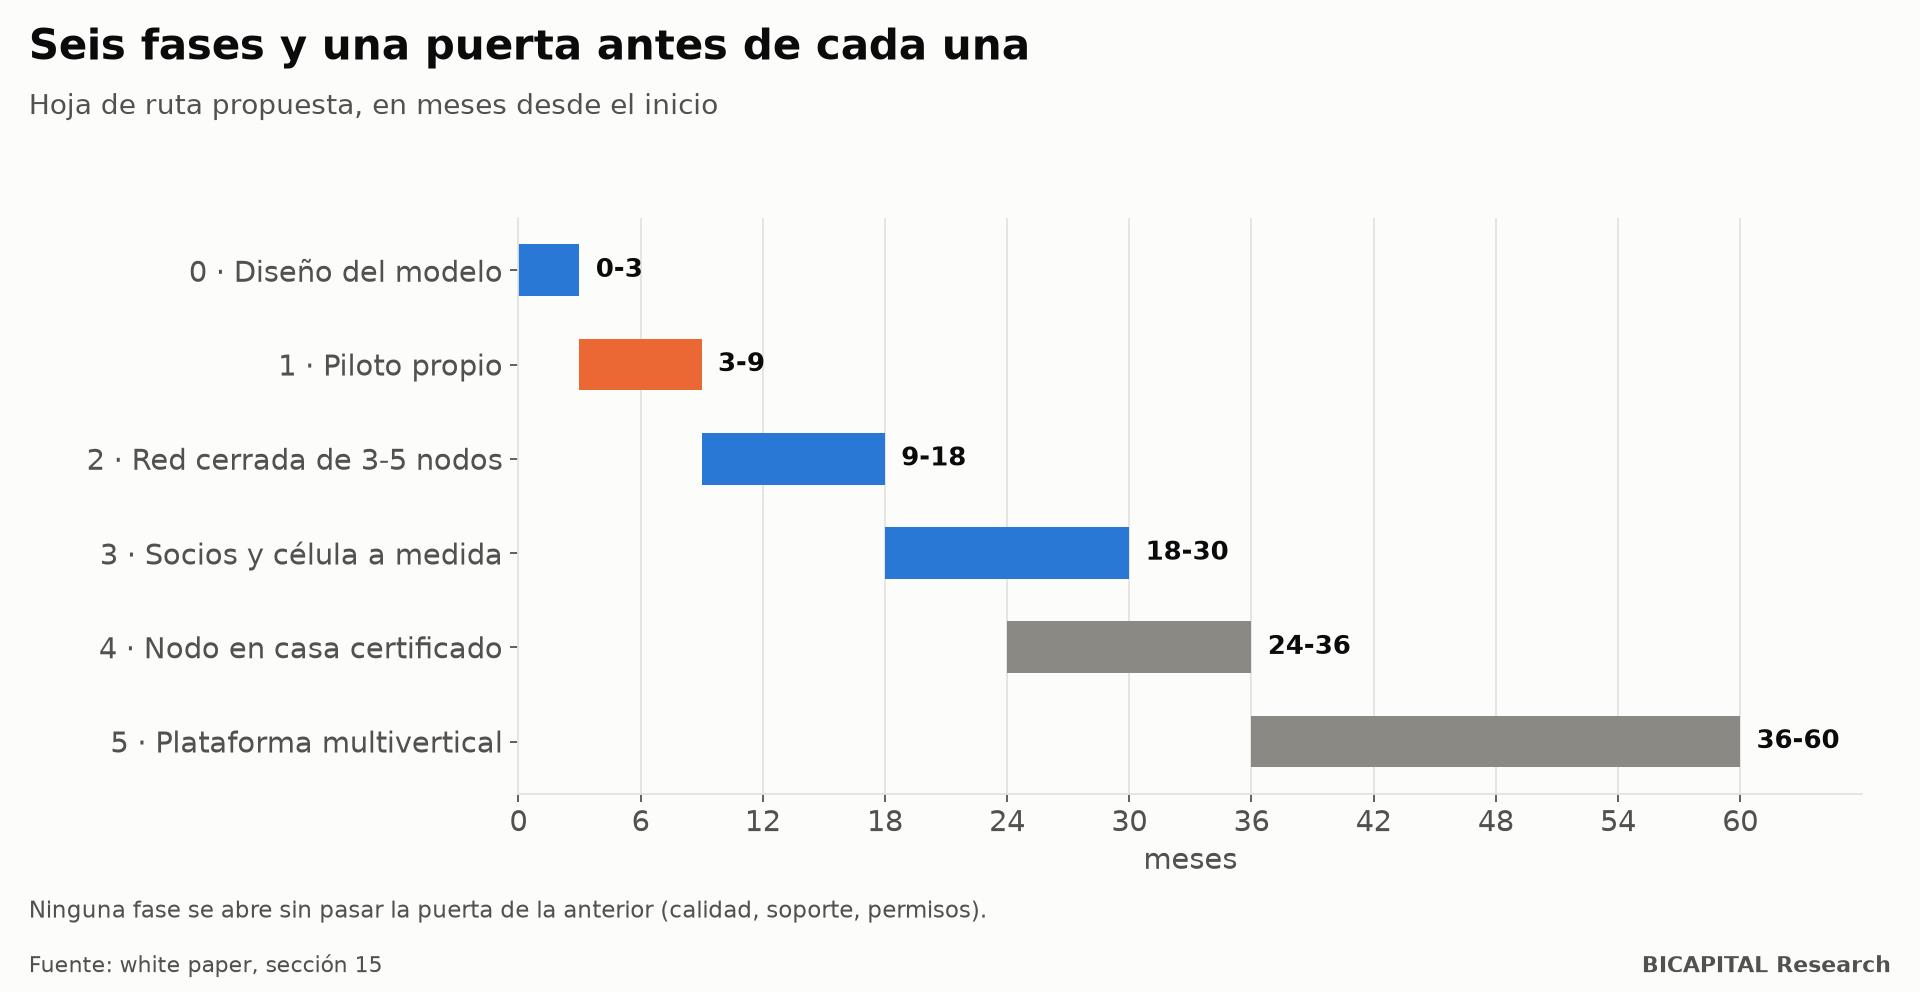
\includegraphics[width=\textwidth]{E02_hoja_de_ruta.png}
\caption{Hoja de ruta de despliegue.}
\label{fig:hojaderuta}
\end{figure}

La figura~\ref{fig:hojaderuta} resume las fases que se detallan a continuación.

\subsubsection*{Fase 0 -- Oficina de diseño del modelo (0--3 meses)}
\begin{itemize}
\item Nombrar líder y equipo núcleo.
\item Definir nomenclatura del sistema y propiedad intelectual.
\item Seleccionar producto piloto y punto de desacople.
\item Mapear proceso actual con tiempos, riesgos y datos.
\item Preparar especificación del intermedio.
\item Validar ruta regulatoria preliminar.
\item Construir P\&L conceptual y criterios de aceptación sin proyectar escala no demostrada.
\item Seleccionar local piloto y canal digital.
\end{itemize}
\etiqueta{Entregables}
\begin{itemize}
\item Mapa de proceso central-local.
\item Especificación de producto intermedio.
\item Layout de nodo v0.
\item URS de demostrador.
\item Matriz regulatoria.
\item Plan de pruebas y KPIs.
\end{itemize}

\subsubsection*{Fase 1 -- Piloto propio (3--9 meses)}
\begin{itemize}
\item Instalar célula con equipos comerciales programables.
\item Integrar MVP de pedidos, lotes, receta y calidad.
\item Operar bajo control directo.
\item Medir demanda, ciclo, limpieza, fallas y delivery.
\item Iterar producto y empaque.
\item Generar manual visual y videos.
\item Obtener permisos y documentación del formato.
\end{itemize}
\begin{caja}{Gate 1}
Producto conforme en condiciones reales; operación repetible; trazabilidad completa; mantenimiento
manejable; demanda suficiente; cero ambigüedades críticas de permiso.
\end{caja}

\subsubsection*{Fase 2 -- Red cerrada de 3 a 5 nodos (9--18 meses)}
\begin{itemize}
\item Instalar nodos propios en zonas distintas.
\item Probar rutas, balance de inventario y asignación.
\item Crear soporte remoto y stock de repuestos.
\item Comparar desempeño entre operadores.
\item Cerrar diseño de célula v1 y URS OEM.
\item Introducir liquidación y contabilidad por nodo.
\end{itemize}
\begin{caja}{Gate 2}
La carga central de soporte por nodo debe disminuir; la variación de calidad entre nodos debe estar
dentro de especificación; la logística debe tener densidad suficiente.
\end{caja}

\subsubsection*{Fase 3 -- Socios controlados y célula OEM (18--30 meses)}
\begin{itemize}
\item Seleccionar 2--5 socios con perfil operativo.
\item Instalar célula v1 bajo arrendamiento.
\item Ejecutar FAT/SAT y homologar proveedor.
\item Aplicar auditoría de sitio y capacitación.
\item Probar contrato de suministro, software y mantenimiento.
\item Validar economía del operador con datos reales.
\end{itemize}
\begin{caja}{Gate 3}
El socio opera sin presencia diaria del fundador; calidad, pagos, inventario y mantenimiento se controlan
por sistema.
\end{caja}

\subsubsection*{Fase 4 -- Nodo domiciliario certificado (24--36 meses)}
\begin{itemize}
\item Seleccionar proceso de menor riesgo y operadores con sitio compatible.
\item Obtener criterios y permisos antes de instalar.
\item Utilizar célula cerrada y área segregada.
\item Limitar menú, horarios y radio.
\item Aumentar telemetría y auditoría inicial.
\item Evaluar aceptación vecinal, entrega y seguridad.
\end{itemize}
\begin{caja}{Gate 4}
El formato domiciliario demuestra cumplimiento, experiencia del cliente y costo de soporte equivalente o
mejor que el microlocal.
\end{caja}

\subsubsection*{Fase 5 -- Plataforma multivertical (36--60 meses)}
\begin{itemize}
\item Separar plataforma de producto.
\item Reutilizar SORP, contratos, mantenimiento y financiación.
\item Agregar segunda vertical con alta reutilización de logística o célula.
\item Crear catálogo homologado de módulos.
\item Expandir a Guayaquil/Cuenca según demanda y soporte.
\item Explorar licenciamiento B2B y white label.
\end{itemize}

\subsection{Equipo mínimo}
{\small
\begin{xltabular}{\textwidth}{@{}P{4.4cm}L@{}}
\toprule
\textbf{Rol} & \textbf{Responsabilidad inicial}\\ \midrule
CEO/arquitecto de negocio & Tesis, capital, socios, producto y expansión.\\
Líder de producto/proceso & Punto de desacople, especificación, rendimiento y validación.\\
Responsable técnico-sanitario & BPM, regulación, calidad, laboratorio y documentación.\\
Ingeniería mecatrónica & URS, integración, seguridad, FAT/SAT y mantenimiento.\\
Software/IoT & MVP, edge, datos, trazabilidad e integraciones.\\
Operaciones/logística & Hub, rutas, inventario, nodos y SOP.\\
Comercial/growth & Demanda digital, marca, ubicaciones y operadores.\\
Legal/tributario externo & Contratos, permisos, importación, laboral y privacidad.\\
\bottomrule
\end{xltabular}}

% =====================================================================
\section{Viabilidad estratégica y hueco de mercado}

\lead{La conclusión no es que toda manufactura vaya a distribuirse. La conclusión es que existe una clase
de procesos donde la combinación de intermedio central, terminación local y automatización compacta
puede crear una ventaja estructural. Ecuador es un mercado adecuado para probarla porque concentra
demanda urbana, posee cadenas agroalimentarias, tiene costos logísticos relevantes y permite comenzar con
una operación existente.}

\subsection{Evidencia que apoya la tesis}
\begin{itemize}
\item \textbf{Centralización ya probada.} Las cocinas centrales/commissary son una práctica conocida para
estandarizar y abastecer múltiples puntos; investigaciones sobre el modelo reportan beneficios de costo,
calidad e integración, aunque el resultado depende del diseño de la cadena. [EXT-27]
\item \textbf{Canal de entrega maduro.} Las plataformas de delivery y la demanda digital permiten crear
puntos sin salón; el problema operativo de asignar cocción y reparto es objeto de investigación y
optimización. [EXT-28]
\item \textbf{Automatización comercial.} Robots de fritura, cocedores digitales, equipos de empaque,
visión y cobots ya existen. [EXT-12][EXT-15][EXT-16][EXT-22][EXT-23]
\item \textbf{Ecosistema chino.} La escala industrial de China reduce barreras para obtener módulos y
personalización OEM. [EXT-01][EXT-02]
\item \textbf{Base local.} Ecuador tiene productores de alimentos con plantas, marcas, operación,
clientes y programas BPM que pueden servir de primer vertical.
\end{itemize}

\subsection{Hueco de mercado}
La mayoría de actores resuelve una sola capa: fabricantes de maquinaria venden equipos; integradores
automatizan plantas; franquicias venden marca y manuales; dark kitchens alquilan espacio; delivery agrega
demanda; software gestiona restaurantes; fabricantes de alimentos venden producto terminado. El hueco es
una empresa que venda el sistema completo de producción distribuida: producto intermedio + célula +
software + suministro + calidad + mantenimiento + canal + operador.

\subsection{Evaluación fría}
{\small
\begin{xltabular}{\textwidth}{@{}P{3.6cm}P{3.4cm}L@{}}
\toprule
\textbf{Dimensión} & \textbf{Evaluación} & \textbf{Comentario}\\ \midrule
\endhead
Necesidad de mercado & Favorable & Reducir inversión y complejidad del punto es valioso para operadores y cadenas.\\
Disponibilidad tecnológica & Favorable & Los módulos existen; la integración y limpieza siguen siendo trabajo real.\\
Ventaja de Ecuador & Selectiva & Agroalimentos, camarón, frutas, cacao y operación local; mercado menor exige expansión ordenada.\\
Barreras de entrada & Medias-Altas & Proceso, datos, permisos, logística, soporte y capital de equipos; no solo software.\\
Escalabilidad & Alta después de estandarizar & La replicación puede ser rápida, pero el soporte físico crece si la célula no es robusta.\\
Riesgo regulatorio & Alto en nodos domiciliarios & Debe resolverse antes de convertirlo en promesa comercial.\\
Riesgo de demanda & Alto por ubicación & Cada nodo necesita densidad; el marketing central no crea demanda infinita.\\
Potencial de plataforma & Alto & Software, mantenimiento, leasing y homologación son reutilizables.\\
Prioridad & Construir & La idea justifica un piloto profesional, no una expansión inmediata.\\
\bottomrule
\end{xltabular}}

\subsection{Oportunidades de negocio derivadas}
{\small
\begin{xltabular}{\textwidth}{@{}P{4.4cm}P{3.6cm}L@{}}
\toprule
\textbf{Oportunidad} & \textbf{Cliente} & \textbf{Modelo}\\ \midrule
\endhead
Red propia de alimentos & Consumidor final & Margen de producto + canal.\\
Microfranquicias automatizadas & Operadores & Suministro + leasing + software + regalía.\\
Células OEM para terceros & Cadenas y fabricantes & Proyecto + mantenimiento + software.\\
Factory OS vertical & Redes de nodos & SaaS + integración.\\
Leasing de equipos & Operadores y pymes & Canon + servicio.\\
Mantenimiento multimarca & Importadores y redes & Suscripción + repuestos.\\
Calidad remota y trazabilidad & Fabricantes & Software + auditoría.\\
Logística de intermedios & Marcas y franquicias & Servicio por ruta/volumen.\\
White label de microproducción & Marcas de terceros & Maquila + red de nodos.\\
Financiación y seguro de células & Operadores & Alianza financiera + fee.\\
\bottomrule
\end{xltabular}}

\subsection{Decisión recomendada}
\begin{caja}{Recomendación}
Constituir el proyecto como una plataforma de ingeniería y operación de redes productivas. Usar un
productor de alimentos existente como primer vertical y activo de aprendizaje. Desarrollar un nodo frío
comercial y un demostrador de snack caliente. No vender todavía la narrativa de “cientos de casas”;
construir primero el estándar que hará posible certificar y controlar esas casas.
\end{caja}

% =====================================================================
\section{Visión 2035 y narrativa para socios}

\lead{La visión a 2035 no depende de que existan humanoides perfectos. Depende de que cada generación de
célula absorba más tareas y que el sistema pueda actualizar recetas, diagnosticar fallas y coordinar
capacidad. La red se vuelve más autónoma por acumulación modular.}

\subsection{Evolución esperada}
{\small
\begin{xltabular}{\textwidth}{@{}P{2cm}LLL@{}}
\toprule
\textbf{Horizonte} & \textbf{Célula} & \textbf{Operador} & \textbf{Software}\\ \midrule
2026--2028 & Equipos programables conectados; carga y empaque humanos. & Ejecuta, limpia y resuelve excepciones. & Pedidos, receta, lotes, calidad y soporte.\\
2028--2031 & Alimentación por cartuchos, visión, dosificación y autolimpieza parcial. & Repone, empaca y atiende clientes. & Forecast, mantenimiento, visión y asignación dinámica.\\
2031--2035 & Células multicategoría, robots compactos y cambio rápido. & Supervisa varias células y excepciones. & Gemelo operativo, agentes y optimización local.\\
Más allá & Mayor manipulación general y logística autónoma. & Gestor de nodo/red. & Mercado de recetas/capacidad y manufactura bajo demanda.\\
\bottomrule
\end{xltabular}}

\subsection{Narrativa de 90 segundos}
\begin{caja}{Pitch}
Hoy una franquicia obliga a cada operador a comprar una cocina, contratar personal, conseguir insumos,
aprender procesos y asumir inventario. Nosotros hacemos lo contrario. Concentramos compras, formulación,
calidad y procesos complejos en un hub. Luego enviamos un producto intermedio a células automatizadas
instaladas cerca del consumidor. El operador necesita poco espacio, poco capital y pocas tareas. El
software asigna pedidos, carga recetas, controla lotes, registra calidad y coordina logística. Empezamos
con alimentos en Ecuador porque es posible empezar sobre una operación productiva existente; pero la
plataforma puede extenderse a otras industrias. No vendemos una máquina. Construimos una red de
producción distribuida.
\end{caja}

\subsection{Mapa de expansión}
La empresa puede expandirse en dos direcciones: por verticales (alimentos fríos, snacks calientes,
bebidas, limpieza, cosmética, impresión, repuestos) y por capas de plataforma (software, mantenimiento,
leasing, homologación, logística de intermedios), que se reutilizan entre verticales.

\subsection{Preguntas que un socio debe hacer}
\begin{itemize}
\item ¿Cuál es el primer producto y por qué puede sostener utilización?
\item ¿Cuál es exactamente el intermedio y qué vida útil tiene?
\item ¿Qué proceso se elimina del nodo y cuánto espacio ahorra?
\item ¿Qué tarea automatiza la célula y cuál sigue siendo humana?
\item ¿Qué permiso necesita cada tipo de establecimiento?
\item ¿Cómo se mantiene el equipo a 300 km?
\item ¿Qué parte del software es imprescindible para el MVP?
\item ¿Qué datos demuestran que la red mejora con cada nodo?
\item ¿Quién es dueño de la célula y qué pasa si el operador sale?
\item ¿Cuál es la ventaja que un competidor no puede copiar comprando la misma máquina?
\end{itemize}

\subsection{Cierre}
La oportunidad no consiste en reemplazar una fábrica grande por miles de cocinas informales. Consiste en
diseñar una red industrial donde la complejidad se concentra, la capacidad se distribuye y la ejecución
se vuelve auditable. El hub fabrica conocimiento y producto intermedio; la célula convierte ese
conocimiento en producción local; el software convierte miles de ciclos en una sola empresa. Esa
combinación puede reducir la inversión del operador, acercar la producción al cliente y permitir una
expansión que las franquicias tradicionales no alcanzan.

% =====================================================================
\clearpage
\section*{Anexos}
\addcontentsline{toc}{section}{Anexos}

\subsection*{Anexo A. Checklist de selección de producto}
\addcontentsline{toc}{subsection}{Anexo A. Checklist de selección de producto}
{\small
\begin{xltabular}{\textwidth}{@{}P{0.6cm}P{2.6cm}LP{1.6cm}P{2.6cm}@{}}
\toprule
\textbf{\#} & \textbf{Dimensión} & \textbf{Pregunta} & \textbf{Puntaje} & \textbf{Evidencia}\\ \midrule
\endhead
1 & Demanda & ¿Existe frecuencia suficiente en un radio pequeño? & 0 / 1 / 2 & \\
2 & Intermedio & ¿Puede transportarse y almacenarse de forma segura? & 0 / 1 / 2 & \\
3 & Valor local & ¿La terminación mejora frescura, tiempo o personalización? & 0 / 1 / 2 & \\
4 & Ciclo & ¿El tiempo final cabe en la promesa de servicio? & 0 / 1 / 2 & \\
5 & Célula & ¿Puede operar con equipo compacto y modular? & 0 / 1 / 2 & \\
6 & Operador & ¿Una persona sin oficio especializado puede ejecutar? & 0 / 1 / 2 & \\
7 & Limpieza & ¿La limpieza es corta, clara y auditable? & 0 / 1 / 2 & \\
8 & Calidad & ¿Se pueden medir variables críticas automáticamente? & 0 / 1 / 2 & \\
9 & Regulación & ¿Existe ruta de permiso razonable? & 0 / 1 / 2 & \\
10 & Logística & ¿Una ruta consolidada sirve a varios nodos? & 0 / 1 / 2 & \\
11 & Portafolio & ¿La misma célula produce variantes sin gran cambio? & 0 / 1 / 2 & \\
12 & Mantenimiento & ¿Los fallos se resuelven por módulo? & 0 / 1 / 2 & \\
13 & Economía & ¿El nodo puede sostener costos con demanda real? & 0 / 1 / 2 & \\
14 & Defensa & ¿La plataforma acumula datos, proceso o red? & 0 / 1 / 2 & \\
\bottomrule
\end{xltabular}}
\noindent Puntaje sugerido: 0 = no demostrado o desfavorable; 1 = plausible con trabajo; 2 = demostrado
o favorable. No seleccionar por puntaje total si existe un gate regulatorio o sanitario en cero.

\subsection*{Anexo B. Plantilla de RFQ para célula OEM}
\addcontentsline{toc}{subsection}{Anexo B. Plantilla de RFQ para célula OEM}
{\small
\begin{xltabular}{\textwidth}{@{}P{4.4cm}L@{}}
\toprule
\textbf{Sección} & \textbf{Contenido requerido}\\ \midrule
\endhead
1. Información del proyecto & Producto, país de instalación, objetivo, fotos, videos y NDA.\\
2. Especificación del producto & Material, dimensiones, temperatura, viscosidad, variación, alérgenos, empaque y muestras.\\
3. Capacidad & Órdenes/hora, lote, pico, disponibilidad, cambio de receta y expansión.\\
4. Secuencia & Diagrama paso a paso, tiempos, parámetros, acciones humanas y puntos de control.\\
5. Higiene & Acero, sellos, grado alimentario, desmontaje, lavado, drenaje, CIP y químicos.\\
6. Seguridad & Normas, guardas, E-stop, interlocks, fuego, temperatura, presión y electricidad.\\
7. Automatización & PLC, HMI, servos, recetas, usuarios, alarmas, logs y acceso remoto.\\
8. Integración & API, OPC UA, MQTT, Modbus, Ethernet/IP, formatos y propiedad de datos.\\
9. Utilidades & Voltaje, frecuencia, potencia, aire, agua, drenaje, gas, extracción y ambiente.\\
10. Layout & Dimensiones, peso, puntos de servicio, mantenimiento, acceso y flujo.\\
11. Documentación & Planos, P\&ID, BOM, manual, certificados, backups, código y videos.\\
12. Servicio & Garantía, respuesta, instalación, capacitación, repuestos y soporte remoto.\\
13. FAT & Producto real, número de ciclos, capacidad, conformidad, limpieza, alarmas y datos.\\
14. SAT & Instalación Ecuador, utilidades, integración, capacitación, capacidad y aceptación.\\
15. Oferta & Precio EXW/FOB/CIF, lead time, pagos, empaque, peso, HS code sugerido y validez.\\
\bottomrule
\end{xltabular}}

\subsection*{Anexo C. Checklist de auditoría de nodo}
\addcontentsline{toc}{subsection}{Anexo C. Checklist de auditoría de nodo}
{\small
\begin{xltabular}{\textwidth}{@{}P{3.4cm}L@{}}
\toprule
\textbf{Dominio} & \textbf{Verificación}\\ \midrule
\endhead
Permisos & Permiso vigente, uso de suelo, responsables y documentos visibles.\\
Área & Separación, flujo, superficies, iluminación, ventilación y acceso.\\
Servicios & Agua, drenaje, electricidad, respaldo, extracción y conectividad.\\
Frío & Temperaturas, alarmas, capacidad, limpieza y calibración.\\
Equipo & Guardas, E-stop, sensores, mantenimiento, software y estado.\\
Insumos & Lotes, FEFO, integridad, temperatura y almacenamiento.\\
Operación & Escaneo, receta, límites, secuencia y evidencia.\\
Limpieza & POES, químicos, concentración, registros y verificación.\\
Plagas/residuos & Prevención, contenedores, retiro y evidencias.\\
Personal & Capacitación, higiene, acceso y salud según política.\\
Calidad & Peso, temperatura, fotos, rechazo y producto no conforme.\\
Ciber/datos & Usuarios, dispositivos, red, cámaras, privacidad y sincronización.\\
Cierre & Conciliación, merma, inventario, limpieza y seguridad.\\
\bottomrule
\end{xltabular}}

\subsection*{Anexo D. Estándar mínimo de célula v1}
\addcontentsline{toc}{subsection}{Anexo D. Estándar mínimo de célula v1}
\begin{itemize}
\item Identificación única de célula y nodo.
\item Recetas versionadas y protegidas.
\item Modo producción, limpieza y mantenimiento separados.
\item Escaneo de lote y validación de compatibilidad.
\item Registro de inicio, fin, variables y alarmas.
\item Paro de emergencia e interlocks locales.
\item Operación segura sin nube durante ventana controlada.
\item Exportación de datos y API documentada.
\item Componentes críticos identificados y repuestos disponibles.
\item Manual de instalación, operación, limpieza y mantenimiento.
\item Lista de consumibles y vida útil.
\item FAT y SAT con criterios cuantitativos.
\item Materiales compatibles con producto y limpieza.
\item Diseño sin zonas de atrapamiento o contaminación evitables.
\item Capacidad de diagnóstico remoto con consentimiento y control.
\end{itemize}

\etiqueta{Niveles de autonomía}
{\small
\begin{xltabular}{\textwidth}{@{}P{4.4cm}L@{}}
\toprule
\textbf{Nivel} & \textbf{Descripción}\\ \midrule
A0 -- Manual guiado & El software muestra pasos; equipo no controla receta.\\
A1 -- Ciclo programado & Equipo controla tiempo/temperatura; carga y descarga manual.\\
A2 -- Dosificación/inspección & Carga parcial, dosificación o visión automatizadas.\\
A3 -- Célula integrada & Múltiples módulos coordinados, empaque parcial y autolimpieza.\\
A4 -- Nodo supervisado & Varias células, manipulación y logística interna automáticas; humano por excepción.\\
\bottomrule
\end{xltabular}}

\subsection*{Anexo E. Fuentes y nivel de evidencia}
\addcontentsline{toc}{subsection}{Anexo E. Fuentes y nivel de evidencia}
Clasificación: A = regulador, organismo oficial o investigación académica; B = documentación oficial de
fabricante/empresa; C = fuente comercial o de descubrimiento. Las afirmaciones de proveedores deben
verificarse mediante RFQ, FAT y referencias.

{\small
\begin{xltabular}{\textwidth}{@{}P{1.4cm}P{1cm}L@{}}
\toprule
\textbf{ID} & \textbf{Nivel} & \textbf{Fuente}\\ \midrule
\endhead
EXT-01 & A & International Federation of Robotics. World Robotics 2025: Global Robot Demand in Factories Doubles Over 10 Years. \url{https://ifr.org/ifr-press-releases/news/global-robot-demand-in-factories-doubles-over-10-years}\\
EXT-02 & A & International Federation of Robotics. Robot Density Surges / China data, 2026. \url{https://ifr.org/ifr-press-releases/news/robot-density-surges-in-europe-asia-and-americas}\\
EXT-03 & A & ARCSA. Servicios en línea: permisos, BPM, notificaciones y simuladores. \url{https://aplicaciones.controlsanitario.gob.ec/}\\
EXT-04 & A & ARCSA. Normativa Técnica Sanitaria Sustitutiva para Alimentos Procesados, Resolución ARCSA-DE-2022-016-AKRG. \url{https://www.controlsanitario.gob.ec/}\\
EXT-05 & A & ARCSA. Obtención de Notificación Sanitaria de Alimentos Procesados -- fabricación nacional. \url{https://www.controlsanitario.gob.ec/inscripcion-de-notificacion-sanitaria-de-alimentos-procesados-fabricacion-nacional/}\\
EXT-06 & A & ARCSA. Instructivo de permiso de transporte para alimentos procesados. \url{https://www.controlsanitario.gob.ec/}\\
EXT-07 & A & Municipio de Quito. Manual/portal LUAE. \url{https://servicios.quito.gob.ec/luae}\\
EXT-08 & A & Quito Informa. Verificación de uso y compatibilidad del suelo antes de LUAE. \url{https://quitoinforma.quito.gob.ec/2022/09/05/que-hacer-antes-de-solicitar-la-luae/}\\
EXT-09 & A & Servicio de Rentas Internas. Voy a iniciar/emprender mi negocio y RUC. \url{https://www.sri.gob.ec/voy-a-iniciar-mi-negocio}\\
EXT-10 & A & Servicio Nacional de Aduana del Ecuador. Para importar. \url{https://www.aduana.gob.ec/servicio-al-ciudadano/para-importar/}\\
EXT-11 & A & Servicio Ecuatoriano de Normalización. Estado y base legal de reglamentos técnicos. \url{https://www.normalizacion.gob.ec/estado-de-reglamentos-tecnicos-ecuatorianos/}\\
EXT-12 & B & BOTINKIT. AI-driven digital kitchen solutions. \url{https://botinkit.ai/}\\
EXT-13 & B & BOTINKIT OMNI cooking robot. \url{https://botinkit.ai/product/cooking-robot}\\
EXT-14 & B & BOTINKIT case studies. \url{https://botinkit.ai/case/okm}\\
EXT-15 & B & Miso Robotics. AI Kitchen Automation Platform. \url{https://www.misorobotics.com/}\\
EXT-16 & B & Hualian Machinery. Packaging equipment. \url{https://www.hualianmachinery.com/}\\
EXT-17 & B & Hualian. Automatic vacuum thermoforming packaging machine. \url{https://www.hualianmachinery.com/}\\
EXT-18 & B & Techik. X-ray inspection systems for food. \url{https://www.techikgroup.com/}\\
EXT-19 & B & Newamstar. Integrated smart factory and liquid packaging solutions. \url{https://en.newamstar.com/}\\
EXT-20 & B & GELGOOG. Small-scale French fries production line case. \url{https://www.gelgoog.com/news/small-scale-french-fries-line.html}\\
EXT-21 & B & GELGOOG. Tomato processing solution. \url{https://www.gelgoog.com/solutions/tomato.html}\\
EXT-22 & B & DOBOT. Food and beverage cobot applications. \url{https://www.dobot-robots.com/industries/food-beverage.html}\\
EXT-23 & B & JAKA Robotics. Food and beverage applications. \url{https://www.jaka.com/}\\
EXT-24 & B & Hikrobot. Machine vision and mobile robots. \url{https://www.hikrobotics.com/}\\
EXT-25 & B & Pudu Robotics. Service and delivery robots. \url{https://www.pudurobotics.com/en}\\
EXT-26 & C & Pulpo / reporte corporativo sobre consumo digital y expansión de PedidosYa Ecuador 2025. \url{https://pulpo.ec/blog/tecnologia/conoce-como-fue-el-consumo-digital-en-ecuador-en-2025/}\\
EXT-27 & A & Supply Chain Innovation in the Catering Industry: assessment of central kitchen model, 2023. Disponible en ResearchGate.\\
EXT-28 & A & Neria et al. The Restaurant Meal Delivery Problem with Ghost Kitchens, 2024. arXiv:2408.07417.\\
EXT-29 & A & Noh et al. YORI: Autonomous Cooking System Utilizing a Modular Robotic Kitchen, 2024. arXiv:2405.11094.\\
EXT-30 & A & Sierla et al. Automatic Assembly Planning based on Digital Product Descriptions, 2021. arXiv:2104.06509.\\
EXT-31 & A & Liu et al. A Food Package Recognition and Sorting System Based on Structured Light and Deep Learning, 2023. arXiv:2309.03704.\\
\bottomrule
\end{xltabular}}

\etiqueta{Nota metodológica}
Este documento separa evidencia de hipótesis. Los datos regulatorios se basan en portales y documentos
oficiales consultados en julio de 2026, pero deben verificarse antes de cada implementación. Las
capacidades de equipos se basan en documentación de fabricantes y requieren validación independiente.
Los rangos de CAPEX son categorías de planificación y no sustituyen cotizaciones. Los casos de uso son
diseños estratégicos; su factibilidad final depende de pruebas de producto, vida útil, demanda, permisos,
instalación y unit economics.

\subsection*{Anexo F. Resumen de recomendaciones}
\addcontentsline{toc}{subsection}{Anexo F. Resumen de recomendaciones}
{\small
\begin{xltabular}{\textwidth}{@{}P{4.2cm}L@{}}
\toprule
\textbf{Decisión} & \textbf{Recomendación}\\ \midrule
Nombre del proyecto & Usar “Sistema de Producción Distribuida Automatizada” como descriptor; definir marca después.\\
Primer vertical & Helado y postres fríos sobre un productor existente.\\
Segundo demostrador & Snack congelado de terminación automática.\\
Primer formato de nodo & Microlocal/corner propio; domicilio después de ruta regulatoria.\\
Propiedad de célula & Central o vehículo de leasing.\\
Software MVP & Pedidos, lotes, receta, ciclo, calidad, inventario y trazabilidad.\\
Estrategia China & URS $\rightarrow$ RFQ $\rightarrow$ FAT $\rightarrow$ SAT; no compra por catálogo sin prueba.\\
Estrategia de expansión & 3--5 nodos cerrados antes de microfranquiciar.\\
Moat & Proceso + datos + red + mantenimiento + software + suministro.\\
Próxima acción & Taller de descomposición del producto piloto y especificación del intermedio.\\
\bottomrule
\end{xltabular}}

\begin{caja}{Frase final}
No queremos que cada operador construya una fábrica. Queremos entregar una capacidad productiva lista,
controlada y conectada. La central hace difícil lo difícil; la célula hace repetible lo local; la red
convierte esa repetición en escala.
\end{caja}

\end{document}


